\documentclass[11pt,a4paper]{article}
\usepackage[utf8]{inputenc}
\usepackage[german]{babel}
\usepackage[T1]{fontenc}
\usepackage{amsmath}
\usepackage{amsfonts}
\usepackage{amssymb}
\usepackage{graphicx}
\usepackage[margin=1.25cm]{geometry} % Puts the same margin on all borders of the document

% Packages

\usepackage{hyperref} % Generate hyperlinks to referenced items
\usepackage{adjustbox} % Used to change parameters in \includegraphics[scale=•]{•}
\usepackage{enumitem} % Provides several options for lists
\usepackage{verbatim} % Package to use \begin{comment}
\usepackage{pdfpages} % Used to import PDF pages
\usepackage{multirow} % Allows us to have a single cell in a table span multiple rows
\usepackage{makecell} % Allows us to format multiple lines in a single cell
\usepackage{minted} % Used to syntax highlight code
\usepackage{xcolor}  % Gives access to coloring text
\usepackage{longtable} % Allows us to create a table over multiple pages
\usepackage{float} % Improved placement of floating items
\usepackage{pdfpages} % Used to import pdf pages
\usepackage{booktabs} % Used for horizontal lines instead of \hline



% Settings

\graphicspath{{./files/}} % Sets path for files to the files folder in the same directory

\hypersetup{
    colorlinks=false, %set true if you want colored links
    linktoc=all,     %set to all if you want both sections and subsections linked
    linkcolor=blue,  %choose some color if you want links to stand out
}

\begin{titlepage}
  \title{Algorithmen und Datenstrukturen} % document_name-type_of_document
  \author{Jonas Milkovits}
  \date{Last Edited: \today}
\end{titlepage}

\begin{document}

\pagenumbering{gobble}
\maketitle
\pagenumbering{roman} % i, ii, iii on beginning pages, that don't have content
\tableofcontents
\clearpage
\pagenumbering{arabic} % 1,2,3 on content pages


\section{Einleitung}
\subsection{Probleme in der Informatik}
\begin{itemize}
    \item Problem im Sinne der Informatik
	    \begin{itemize}
          	\item Enthält eine Beschreibung der Eingabe 
          	\item Enthält eine Beschreibung der Ausgabe
          	\item Gibt \textbf{keinen} Übergang von Eingabe und Ausgabe an
          	\item z.B.: Finde den kürzesten Weg zwischen zwei Orten
	    \end{itemize}
	
    \item Probleminstanzen
        \begin{itemize}
          	\item Probleminstanz ist eine konkrete Eingabenbelegung, für die entsprechende Ausgabe gewünscht ist
          	\item z.B.: Was ist der kürzeste Weg vom Audimax in die Mensa?
    	\end{itemize}

\end{itemize}

\subsection{Definitionen für Algorithmen}
\begin{itemize}
    \item Begriff des Algorithmus
        \begin{itemize}
        	\item Endliche Folge von Rechenschritten, der eine Ausgabe in eine Eingabe verwandelt 
        \end{itemize}
        
    \item Anforderungen an Algorithmen
        \begin{itemize}
            \item Spezifizierung der Eingabe und Ausgabe 
              \begin{itemize}
                    \item Anzahl und Typen aller Elemente ist definiert
              \end{itemize}
          \item Eindeutigkeit
              \begin{itemize}
                    \item Jeder Einzelschritt ist klar definiert und ausführbar 
                    \item Die Reihenfolge der Einzelschritte ist festgelegt
              \end{itemize}
            \item Eindlichkeit
              \begin{itemize}
                    \item Notation hat eine endliche Länge
              \end{itemize}
        \end{itemize}

    \item Eigenschaften von Algorithmen
        \begin{itemize}
	    	\item Determiniertheit
	    		\begin{itemize}
	    			\item Für gleiche Eingabe stets die gleiche Ausgabe (andere mögliche Zwischenzustände)
	    		\end{itemize}
	    	\item Determinismus
	    		\begin{itemize}
	    			\item Für gleiche Eingabe stets identische Ausführung und Ausgabe
	    		\end{itemize}
	    	\item Terminierung
	    		\begin{itemize}
	    			\item Algorithmus läuft für jede Eingabe nur endlich lange
	    		\end{itemize}
	    	\item Korrektheit
	    		\begin{itemize}
	    			\item Algorithmus berechnet stets die spezifizierte Ausgabe (falls dieser terminiert)
	    		\end{itemize}
	    	\item Effizienz
	    		\begin{itemize}
	    			\item Sparsamkeit im Ressourcenverbrauch (Zeit, Speicher, Energie,...)
	    		\end{itemize}
	    \end{itemize}
\end{itemize}

\pagebreak

\section{Sortieren}
\subsection{Einführung ins Sortieren}
    \begin{itemize}
        \item \textbf{Das Sortierproblem}
            \begin{itemize}
                \item Ausgangspunkt: Folge von Datensätzen $D_1,D_2,...,D_n$
                \item Zu sortierende Elemente hei\ss en auch Schlüssel(werte)
                \item Ziel: Datensätze so anzuordnen, dass die Schlüsselwerte sukzessive ansteigen/absteigen
                \item Bedingung: Schlüsselwerte müssen vergleichbar sein
                \item Durchführung:
                    \begin{itemize}
                        \item Eingabe: Sequenz von Schlüsselwerten $<a_1,a_2,...,a_n>$
                        \item Engabe ist eine \textbf{Instanz} des Sortierproblems
                        \item Ausgabe: Permutation $<a_1', a_2', ..., a_n'>$ derselben Folge mit Eigenschaft $a_1' \leq ... \leq a_n'$
                    \end{itemize}
                \item Algorithmus \textbf{korrekt}, wenn dieser das Problem für alle Instanzen löst
            \end{itemize}

        \item \textbf{Exkurs: Totale Ordnung}
            \begin{itemize}
                \item Sei $M$ eine nicht leere Menge und $\leq \subseteq MxM$ eine binäre Relation auf $M$
                \item Das Paar $(M, \leq)$ hei\ss t genau dann totale Relation auf der Menge $M$, wenn Folgendes erfüllt ist:
                    \begin{itemize}
                        \item Reflexivität: $\forall x \in M: x \leq x$
                        \item Transitivität: $\forall x,y,z \in M: x \leq y \land y \leq z \Rightarrow x \leq z$
                        \item Antisymmetrie: $\forall x,y \in M: x \leq y \land y \leq x \Rightarrow x = y$
                        \item Totalität: $\forall x,y \in M: x \leq y \lor y \leq x$
                    \end{itemize}
                \item z.B.: $\leq$ Ordnung auf natürlichen Zahlen bildet eine totale Ordnung ($1 \leq 2 \leq 3 ...$)
                \item z.B.: Lexikographische Ordnung $\leq_{lex}$ ist eine totale Ordnung ($A \leq B \leq C ...$)
            \end{itemize}
        
        \item \textbf{Vergleichskriterien von Sortieralgorithmen}
            \begin{itemize}
                \item Berechnungsaufwand $O(n)$
                \item Effizient: Best Case vs Average Case vs Worst Case
                \item Speicherbedarf:
                    \begin{itemize}
                        \item in-place (in situ): Zusätzlicher Speicher von der Eingabegrö\ss e unabhängig
                        \item out-of-place: Speichermehrbedarf von Eingabegrö\ss e abhängig
                    \end{itemize}
                \item Stabilität: Stabile Verfahren verändern die Reihenfolge von äquivalenten Elementen nicht
                \item Anwendung als Auswahlfaktor: 
                    \begin{itemize}
                        \item Hauptoperationen beim Sortieren: Vergleiche und Vertausche
                        \item Diese Operationen können sehr teuer oder sehr günstig sein, je nach Aufwand
                        \item Anpassung des Verfahrens abhängig von dem Aufwand dieser Operationen
                    \end{itemize}    
            \end{itemize}
    \end{itemize}    

    \pagebreak

\subsection{Analyse von Algorithmen - Teil 1} 
    \begin{itemize}

        \item \textbf{Schleifeninvariante (SIV)}
            \begin{itemize}
                \item Sonderform der Invariante 
                \item Am Anfang/Ende jedes Schleifendurchlaufs und vor/nach jedem Schleifendurchlauf gültig
                \item Wird zur Feststellung der Korrektheit von Algorithmen verwendet
                \item Eigenschaften: 
                    \begin{itemize}
                        \item Initialisierung: Invariante ist vor jeder Iteration wahr
                        \item Fortsetzung: Wenn SIV vor der Schleife wahr ist, dann auch bis Beginn der nächsten Iteration
                        \item Terminierung: SIV liefert bei Schleifenabbruch, helfende Eigenschaft für Korrektheit
                    \end{itemize}
                \item Beispiel für Umsetzung: \hyperref[insSortSiv]{\textcolor{red}{Insertion Sort - SIV}}
            \end{itemize}
        
        \item \textbf{Laufzeitanalyse}
            \begin{itemize}
                \item Aufstellung der Kosten und Durchführungsanzahl für jede Zeile des Quelltextes
                \item Beachte: Bei Schleifen wird auch der Aufruf gezählt, der den Abbruch einleitet 
                \item Beispiel für Umsetzung: \hyperref[insSortLaufzeit]{\textcolor{red}{Insertion Sort - Laufzeit}}
                \item Zusätzliche Überprüfung des \texttt{Best Case, Worst Case} und \texttt{Average Case}
            \end{itemize}

        \item \textbf{Effizienz von Algorithmen}
            \begin{itemize}
                \item Effizienzfaktoren
                    \begin{itemize}
                        \item Rechenzeit (Anzahl der Einzelschritte)
                        \item Kommunikationsaufwand 
                        \item Speicherplatzbedarf
                        \item Zugriffe auf Speicher
                    \end{itemize}
                \item Laufzeit hängt von versch. Faktoren ab
                    \begin{itemize}
                        \item Länge der Eingabe
                        \item Implementierung der Basisoperationen
                        \item Takt der CPU 
                    \end{itemize}
            \end{itemize}

    \end{itemize}

\subsection{Analyse von Algorithmen - Teil 2}
    \begin{itemize}
        \item \textbf{Komplexität}
            \begin{itemize}
                \item Abstrakte Rechenzeit $T(n)$ ist abhängig von den Eingabedaten
                \item Übliche Betrachtungsweise der Rechenzeit ist asymptotische Betrachtung
            \end{itemize}
        
        \item \textbf{Asymptotik}
            \begin{itemize}
                \item Annäherung an einer sich ins Unendliche verlaufende Kurve
                \item z.B.: $f(x) = \frac{1}{x} + x$ | Asymptote: $g(x)=x$ | ($\frac{1}{x}$ läuft gegen Null)
            \end{itemize}
        
        \item \textbf{Asymptotische Komplexität}
            \begin{itemize}
                \item Abschätzung des zeitlichen Aufwands eines Algorithmus in Abhängigkeit einer Eingabe
                \item Beispiel für Umsetzung: \hyperref[insSortLaufzeitTheta]{\textcolor{red}{Insertion Sort - Laufzeit $\Theta$}}
            \end{itemize}

        \item \textbf{Asymptotische Notation}
            \begin{itemize}
                \item Betrachtung der Laufzeit $T(n)$ für sehr gro\ss e Eingaben $n \in \mathbb{N}$
                \item Komplexität ist unabhängig von konstanten Faktoren und Summanden
                \item Nicht berücksichtigt: Rechnergeschwindigkeit / Initialisierungsauswände
                \item Komplexitätsmessung via Funktionsklasse ausreichend
                    \begin{itemize}
                        \item Verhalten des Algorithmus für gro\ss e Problemgrö\ss en
                        \item Veränderung der Laufzeit bei Verdopplung der Problemgrö\ss e
                    \end{itemize}
            \end{itemize}
        
        \item \textbf{Gründe für die Nutzung der theoretischen Betrachtung statt der Messung der Laufzeit }
            \begin{itemize}
                \item Vergleichbarkeit
                    \begin{itemize}
                        \item Laufzeit abhängig von konkreter Implementierung und System
                        \item Theoretische Betrachung ist frei von Abhängigkeiten und Seiteneffekten
                        \item Theoretische Betrachtung lässt direkte Vergleichbarkeit zu
                    \end{itemize}
                
                \item Aufwand
                    \begin{itemize}
                        \item Wieviele Testreihen?
                        \item In welcher Umgebung?
                        \item Messen führt in der Ausführung zu hohem, praktischen Aufwand
                    \end{itemize}
                
                \item Komplexitätsfunktion
                    \begin{itemize}
                        \item Wachstumsverhalten ausreichend
                        \item Praktische Evaluation mit Zeiten nur für Auswahl von Systemen mögliche
                        \item Theoretischer Vergleich (Funktionsklassen) hat ähnlichen Erkenntnisgewinn
                    \end{itemize}
            \end{itemize}
    \end{itemize}

\subsection{Analyse von Algorithmen - Teil 3}
    \begin{itemize}
        \item \textbf{$\Theta$-Notation}
            \begin{itemize}
                \item $\Theta$-Notation beschränkt eine Funktion asymptotisch von oben und unten
                \item Funktionen $f,g: \mathbb{N} \rightarrow \mathbb{R}_{>0}$ ($\mathbb{N}$: Eingabelänge, $\mathbb{R}$: Zeit)
                \item[] 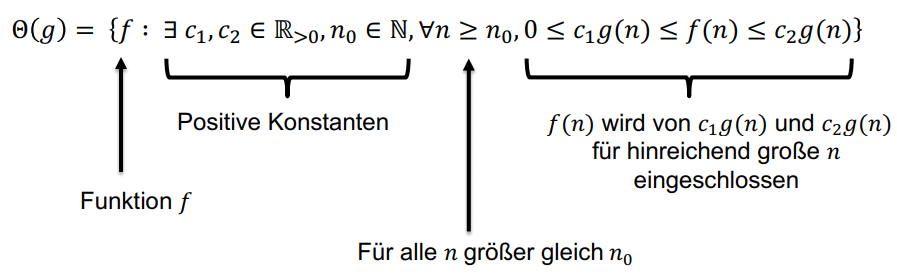
\includegraphics[width=12cm]{thetaNotation.PNG}
                \item $\Theta(g)$ enthält alle $f$, die genauso schnell wachsen wie $g$
                \item Schreibweise: $f \in \Theta(g)$ (korrekt), manchmal auch $f = \Theta(g)$
                \item $g(n)$ ist eine asymptotisch scharfe Schranke von $f(n)$
                \item $f(n)= \Omega(g(n))$ gilt, wenn $f(n) = O(g(n))$ und $f(n)=\Omega(g(n))$ erfüllt sind
                \item[]
                \item[] 
                    \begin{minipage}{0.3\textwidth}
                    \begin{figure}[H]
                        \centering
                        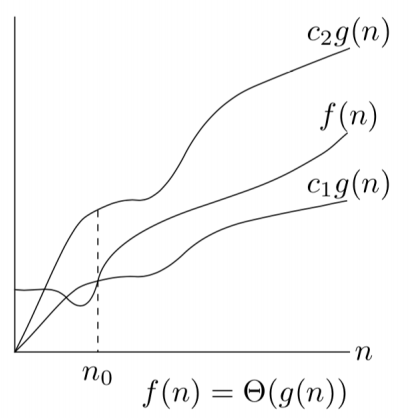
\includegraphics[width=5cm]{thetaNotationGraph.PNG}
                        \caption{Veranschaulichung}
                        \label{}
                    \end{figure}
                    \end{minipage}
                    \begin{minipage}[t]{0.6\textwidth}
                    \vspace{-3cm}
                        \begin{itemize}
                            \item z.B.: $f(n)= \frac{1}{2} n^2 - 3n$ | $f(n) \in \Theta(n^2)$?
                            \item Aus $\Theta(n^2)$ folgt, dass $g(n)=n^2$
                            \item Vorgehen:
                                \begin{itemize}
                                    \item Finden eines $n_0$ und $c_1,c_2$, sodass
                                    \item $c_1*g(n) \leq f(n) \leq c_2*g(n)$ erfüllt ist
                                    \item Konkret: $c_1*n^2 \leq \frac{1}{2} n^2 - 3n \leq c_2*n^2$
                                    \item Division durch $n^2$: $c_1 \leq \frac{1}{2}-\frac{3}{n} \leq c2$
                                    \item Ab $n=7$ positives Ergebnis: $0,0714$ | $n_0 = 7$
                                    \item Deswegen setzen wir $c_1=\frac{1}{14}$
                                    \item Für $n \rightarrow \infty: ~ 0,5$ | $c_2 = 0,5$
                                    \item Natürlich auch andere Konstanten möglich
                                \end{itemize}
                        \end{itemize}
                    \end{minipage}
            \end{itemize}

        \item \textbf{$O$-Notation}
            \begin{itemize}
                \item $O$-Notation beschränkt eine Funktion asymptotisch von oben
                \item[] 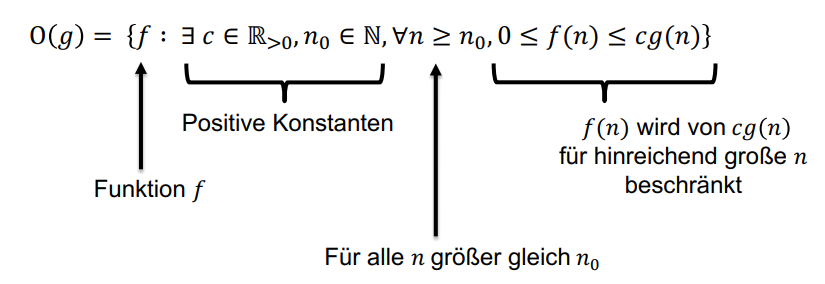
\includegraphics[width=12cm]{oNotation.PNG}
                \item $O(g)$ enthält alle $f$, die höchstens so schnell wie $g$ wachsen
                \item Schreibweise: $f=O(g)$
                \item $f(n)=\Theta(g) \rightarrow f(n) = O(g)$ | $\Theta(g(n)) \subseteq O(g(n))$
                \item Ist $f$ in der Menge $\Theta(g)$, dann auch in der Menge $O(g)$
                \item[]
                \item[] 
                    \begin{minipage}{0.3\textwidth}
                    \begin{figure}[H]
                        \centering
                        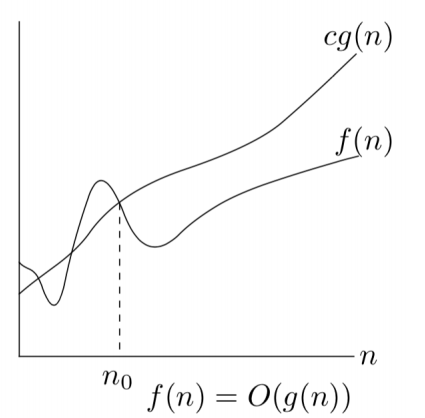
\includegraphics[width=5cm]{oNotationGraph.PNG}
                        \caption{Veranschaulichung}
                        \label{}
                    \end{figure}
                    \end{minipage}
                    \begin{minipage}[t]{0.6\textwidth}
                    \vspace{-3cm}
                        \begin{itemize}
                            \item z.B.: $f(n) = n + 2$ | $f(n) = O(n)$?
                            \item Ja $f(n)$ ist Teil von $O(n)$ für z.B. $c = 2$ und $n_0 = 2$
                        \end{itemize}
                    \end{minipage}
            \end{itemize}
        
        \item \textbf{$O$-Notation Rechenregeln}
            \begin{itemize}
                \item Konstanten: 
                    \begin{itemize}
                        \item $f(n) = a$ mit $a \in \mathbb{R}$ konstante Funktion $\rightarrow$ $f(n) = O(1)$
                        \item z.B. $3 \in O(1)$
                    \end{itemize}
                
                \item Skalare Multiplikation:
                    \begin{itemize}
                        \item $f= O(g)$ und $a \in \mathbb{R}$ $\rightarrow$ $a*f = O(g)$
                    \end{itemize}
                
                \item Addition: 
                    \begin{itemize}
                        \item $f_1 = O(g_1)$ und $f_2 = O(g_2)$ $\rightarrow$ $f_1+f_2= O(max\{g_1,g_2\})$
                    \end{itemize}
                
                \item Multiplikation:
                    \begin{itemize}
                        \item $f_1 = O(g_1)$ und $f_1 = O(g_2)$ $\rightarrow$ $f_1*f_2= O(g_1*g_2)$
                    \end{itemize}
            \end{itemize}
        
        \item \textbf{$\Omega$-Notation}
            \begin{itemize}
                \item $\Omega$-Notation beschränkt eine Funktion asymptotisch von unten
                \item[] 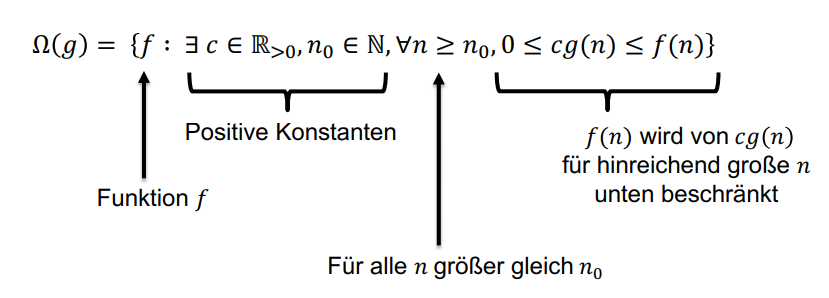
\includegraphics[width=12cm]{omegaNotation.PNG}
                \item $\Omega$-Notation enthält alle $f$, die mindestens so schnell wie $g$ wachsen
                \item Schreibweise: $f = \Omega(g)$
                \item[]
                \item[] 
                    \begin{minipage}{0.3\textwidth}
                    \begin{figure}[H]
                        \centering
                        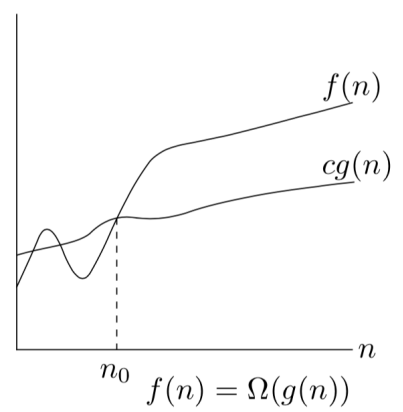
\includegraphics[width=5cm]{omegaNotationGraph.PNG}
                        \caption{Veranschaulichung}
                        \label{}
                    \end{figure}
                    \end{minipage}
                    \begin{minipage}[t]{0.6\textwidth}
                    \vspace{-3cm}
                    \end{minipage}
            \end{itemize}
        
        \item \textbf{Komplexitätsklassen}
            \begin{itemize}
                \item $n$ ist hier die Länge der Eingabe
                \item[] \includegraphics[width=12cm]{komplexitätsklassen.PNG}
                \item Ausführungsdauer, falls eine Operation $n$ genau $1\mu s$ dauert 
                \item[] \includegraphics[width=12cm]{komplexitätsklassenDauer.PNG}
            \end{itemize}
        
        \item Asymptotische Notationen in Gleichungen
            \begin{itemize}
                \item $2n^2 + 3n + 1 = 2n^2 + \Theta(n)$
                \item $\Theta(n)$ fungiert hier als Platzhalter für eine beliebige Funktion $f(n)$ aus $\Theta(n)$
                \item z.B.: $f(n) = 3n + 1$
            \end{itemize}
        
        \item \textbf{$o$-Notation}
            \begin{itemize}
                \item $o$-Notation stellt eine echte obere Schranke dar
                \item Ausschlaggebend ist, dass es für alle $c \in \mathbb{R}_{>0}$ gelten muss
                \item Au\ss erdem $<$ statt $\leq$
                \item z.B.: $2n = o(n^2)$ und $2n^2 \neq o(n^2)$ 
                \item[] 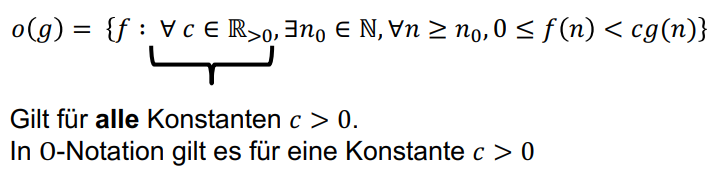
\includegraphics[width=12cm]{oKleinNotation.PNG}
                
            \end{itemize}
        
        \item \textbf{$\omega$-Notation}
            \begin{itemize}
                \item $\omega$-Notation stellt eine echte untere Schranke dar
                \item Ausschlaggebend ist, dass es für alle $c \in \mathbb{R}{>0}$ gelten muss
                \item Au\ss erdem $>$ statt $\geq$
                \item z.B.: $\frac{n^2}{2} = \omega(n)$ und $\frac{n^2}{2} \neq \omega(n^2)$
                \item[] 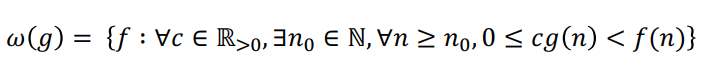
\includegraphics[width=12cm]{omegaKleinNotation.PNG}
            \end{itemize}
    \end{itemize}

\subsection{Insertion Sort}
    \begin{itemize}
        \item \textbf{Idee}
            \begin{itemize}
                \item Halte die linke Teilfolge sortiert
                \item Füge nächsten Schlüsselwert hinzu, indem es an die korrekte Position eingefügt wird
                \item Wiederhole den Vorgang bis Teilfolge aus der gesamten Liste besteht
            \end{itemize}
        
        \item \textbf{Code}
            \begin{itemize}
                \item[]
                 \begin{minted}[autogobble]{c}  
                    FOR j = 1 TO A.length - 1
                      key = A[j]
                      // Füge A[j] in die sortierte Sequenz A[0...j-1] ein
                      i = j - 1
                      WHILE i >= 0 and A[i] > key
                          A[i + 1] = A[i]
                          i = i - 1
                      A[i + 1] = key
                    \end{minted}
            \end{itemize}
            
        \item \textbf{Schleifeninvariante von \texttt{Insertion Sort}} {\label{insSortSiv}} 
            \begin{itemize}
                \item Zu Beginn jeder Iteration der \texttt{for}-Schleife besteht die Teilfolge \texttt{A[0...j-1]} aus den Elementen \\
                der ursprünglichen Teilfolge \texttt{A[0...j-1]} enthaltenen Elementen, allerdings in sortierter Reihenfolge.
            \end{itemize}

        \item \textbf{Korrektheit von \texttt{Insertion Sort}}
            \begin{itemize}
                \item Initialisierung:
                    \begin{itemize}
                        \item   Beginn mit \texttt{j=1}, also Teilfeld \texttt{A[0...j-1]} besteht nur aus einem Element \texttt{A[0]}. \\
                                Dies ist auch das ursprüngliche Element und Teilfeld ist sortiert.
                    \end{itemize}

                \item Fortsetzung:
                    \begin{itemize}
                        \item   Zu zeigen ist, dass die Invariante bei jeder Iteration erhalten bleibt. Ausführungsblock der \texttt{for}-Schleife
                                sorgt dafür, dass \texttt{A[j-1], A[j-2]},... je um Stelle nach rechts geschoben werden bis \texttt{A[j]} korrekt eingefügt wurde. 
                                Teilfeld \texttt{A[0...j]} besteht aus ursprünglichen Elementen und ist sortiert. Inkrementieren von j erhält die Invariante.
                    \end{itemize}

                \item Terminierung: 
                    \begin{itemize}
                        \item   Abbruchbedingung der \texttt{for}-Schleife, wenn \texttt{j > A.length - 1}. Jede Iteration erhöht j.
                                Dann bei Abbruch ist \texttt{j = n } und einsetzen in Invariante liefert das Teilfeld \texttt{A[0...n-1]}
                                welches aus den ursprünglichen Elementen besteht und sortiert ist. Teilfeld ist gesamtes Feld.
                    \end{itemize}

                \item Algorithmus \texttt{Insertion Sort} arbeitet damit korrekt.
                
            \end{itemize}
        
        \item \textbf{Laufzeitanalyse von \texttt{Insertion Sort}} {\label{insSortLaufzeit}}
            \begin{itemize}
                \item[] 
                    \begin{minipage}{0.45\textwidth}
                    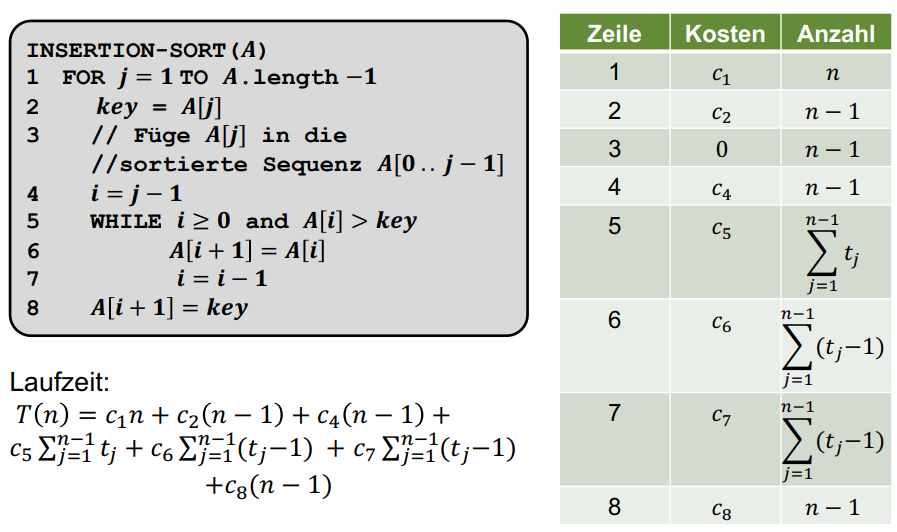
\includegraphics[width=8cm]{insSortLaufzeit.PNG}
                    \end{minipage}
                    \begin{minipage}[t]{0.45\textwidth}
                    \vspace{-2.5cm}
                    \begin{itemize}
                        \item Festlegung der Laufzeit für jede Zeile
                        \item Jede Zeile besitzt gewissen Kosten \texttt{$c_i$}
                        \item Jede Zeile wird $x$ mal durchgeführt 
                        \item $Laufzeit = Anzahl * Kosten$ jeder Zeile
                        \item Schleifen: Abbruchüberprüfung zählt auch
                        \item \texttt{$t_j$}: Anzahl der Abfragen der \texttt{While}-Schleife
                    \end{itemize}
                    \end{minipage}

                \item Warum $n$ in Zeile 1?
                    \begin{itemize}
                        \item Die Überprüfung der Fortführungsbedingung beinhaltet auch die letze Überprüfung 
                        \item Quasi die Überprüfung, durch die die Schleife abbricht
                    \end{itemize}

                \item Warum $\sum^{n-1}_{j=1}$ in Zeile 5?
                    \begin{itemize}
                        \item Aufsummierung aller einzelnen $t_j$ über die Anzahl der Schleifendurchläufe
                        \item Diese ist allerdings $n-1$ und nicht $n$, da die Abbruchüberprüfung dort auch enthalten ist
                    \end{itemize}
                
                \item Warum $t_j-1$ in Zeile 6?
                    \begin{itemize}
                        \item Selbes Argument wie oben, bei $t_j$ ist die Abbruchüberprüfung enthalten
                        \item Deswegen wird die \texttt{while}-Schleife nur $t_j-1$-mal ausgeführt
                    \end{itemize}
                
                \item \texttt{Best Case}
                    \begin{itemize}
                        \item zu sortierendes Feld ist bereits sortiert 
                        \item $t_j$ wird dadurch zu 1, da die \texttt{While}-Schleife immer nur einmal prüft (Abbruch)
                        \item Die zwei Zeilen innerhalb der \texttt{While}-Schleife werden nie ausgeführt
                        \item Durch Umformen ergibt sich, dass die Laufzeit eine lineare Funktion in $n$ ist
                    \end{itemize}
                
                \item \texttt{Worst Case}
                    \begin{itemize}
                        \item zu sortierendes Feld ist umgekehrt sortiert 
                        \item $t_j$ wird dadurch zu $j+1$, da die \texttt{While}-Schleife immer die gesamte Länge prüft
                        \item Durch Umformen ergibt sich, dass die Laufzeit eine quadratische Funktion in $n$ ist ($n^2$)
                    \end{itemize}
                
                \item \texttt{Average Case} 
                    \begin{itemize}
                        \item im Mittel gut gemischt 
                        \item $t_j$ wird dadurch zu $j/2$
                        \item Die Laufzeit bleibt aber eine quadratische Funktion in $n$ ($n^2$)
                    \end{itemize}
            \end{itemize}
        
        \item \textbf{Asymptotische Laufzeitbetrachtung $\Theta$} {\label{insSortLaufzeitTheta}}
            \begin{itemize}
                \item $T(n)$ lässt sich als quadratische Funktion $an^2 + bn + c$ betrachten 
                \item Terme niedriger Ordnung sind für gro\ss e $n$ irrelevant
                \item Deswegen Vereinfachung zu $n^2$ und damit $\Theta(n^2)$
            \end{itemize}
    \end{itemize}
    
\subsection{Bubble Sort}

    \begin{itemize}
        \item \textbf{Idee}
            \begin{itemize}
                \item Vergleiche Paare von benachbarten Schlüsselwerten
                \item Tausche das Paar, falls rechter Schlüsselwert kleiner als linker
            \end{itemize}
        
        \item \textbf{Code}
            \begin{itemize}
                \item[]
                    \begin{minted}[autogobble]{c}  
                    FOR i = 0 TO A.length - 2
                        FOR j = A.length - 1 DOWNTO i + 1
                            IF A[j] < A[j-1]
                                SWAP(A[j], A[j-1])
                    \end{minted}
            \end{itemize}

        \item \textbf{Analyse von \texttt{Bubble Sort}}
            \begin{itemize}
                \item Anzahl der Vergleiche:
                    \begin{itemize}
                        \item Es werden stets alle Elemente der Teilfolge miteinander verglichen
                        \item Unabhängig von der Vorsortierung sind \texttt{Worst} und \texttt{Best Case} identisch
                    \end{itemize}
                
                \item Anzahl der Vertauschungen:
                    \begin{itemize}
                        \item \texttt{Best Case}: 0 Vertauschungen
                        \item \texttt{Worst Case}: $\frac{n^2-n}{2}$ Vertauschungen
                    \end{itemize}
                
                \item Komplexität:
                    \begin{itemize}
                        \item \texttt{Best Case}: $\Theta(n)$
                        \item \texttt{Average Case}: $\Theta(n^2)$
                        \item \texttt{Worst Case}: $\Theta(n^2)$
                    \end{itemize}
            \end{itemize}
        
    \end{itemize}

\pagebreak

\subsection{Selection Sort}
    \begin{itemize}
        \item \textbf{Idee}
            \begin{itemize}
                \item Sortieren durch direktes Auswählen
                \item \texttt{MinSort}: "wähle kleines Element in Array und tausche es nach vorne" 
                \item \texttt{MaxSort}: "wähle größtes Element in Array und tausche es nach vorne" 
            \end{itemize}

        \item \textbf{Code - MinSort}
            \begin{itemize}
                \item[]
                    \begin{minted}[autogobble]{c}
                    FOR i = 0 TO A.length - 2
                        k = i 
                        FOR j = i + 1 TO A.length - 1
                            IF A[j] < A[k]
                                k = j 
                        SWAP(A[i], A[k])
                    \end{minted}
            \end{itemize}
    \end{itemize}

\subsection{Divide-And-Conquer-Ansatz}
    \begin{itemize}
        \item Anderer Ansatz im Gegensatz zu z.B. \texttt{InsertionSort} (inkrementelle Herangehensweise)
        \item Laufzeit ist im schlechtesten Fall immer noch besser als \texttt{InsertionSort}
        \item Prinzip: Zerlege das Problem und löse es direkt oder zerlege es weiter
        \item \textbf{Divide:} 
            \begin{itemize}
                \item Teile das Problem in mehrere Teilprobleme auf
                \item Teilprobleme sind Instanzen des gleichen Problems 
            \end{itemize}
        \item \textbf{Conquer:} 
            \begin{itemize}
                \item Beherrsche die Teilprobleme rekursiv
                \item Falls Teilprobleme klein genug, löse sie auf direktem Weg
            \end{itemize}
        \item \textbf{Combine:} 
            \begin{itemize}
                \item Vereine die Lösungen der Teilprobleme zu Lösung des ursprünglichen Problems
            \end{itemize}
    \end{itemize}

\subsection{Merge Sort} 
    \begin{itemize}
        \item \textbf{Idee} 
            \begin{itemize}
                \item \textbf{Divide:} Teile die Folge aus $n$ Elementen in zwei Teilfolgen von je $\frac{n}{2}$ Elemente auf
                \item \textbf{Conquer:} Sortiere die zwei Teilfolgen rekursiv mithilfe von \texttt{MergeSort}
                \item \textbf{Combine:} Vereinige die zwei sortierten Teilfolgen, um die sortierte Lösung zu erzeugen
            \end{itemize}
        \item \textbf{Code} 
            \begin{itemize}
                \item[]
                    \begin{minted}[autogobble,escapeinside=||]{c}
                    MERGE-SORT (A,p,r)
                    IF p < r
                        q = |$\left \lfloor \texttt{(p+r)/2} \right \rfloor$| // Teilen in 2 Teilfolgen 
                        MERGE-SORT(A,p,q) // Sortieren der beiden Teilfolgen
                        MERGE-SORT(A,q+1,r)
                        MERGE(A,p,q,r) // Vereinigung der beiden sortierten Teilfolgen
                    \end{minted}
                \item[]
                \item[]
                    \begin{minted}[autogobble,escapeinside=||]{c}
                    MERGE(A,p,q,r) // Geteiltes Array an Stelle q
                    |$n_1$| = q - p + 1
                    |$n_2$| = r - q 
                    Let L[0...|$n_1$|] and R[0...|$n_2$|] be new arrays 
                    FOR i = 0 TO |$n_1$| - 1 // Auffüllen der neu erstellten Arrays
                        L[i] = A[p + i]
                    FOR j = 0 TO |$n_2$| - 1
                        R[j] = A[q + j + 1]
                    L[|$n_1$|] = |$\infty$| // Einfügen des Sentinel-Wertes
                    R[|$n_2$|] = |$\infty$|
                    i = 0
                    j = 0
                    FOR k = p TO r  // Eintragweiser Vergleich der Elemente          
                        IF L[i] |$\leq$| R[j]
                            A[k] = L[i] // Sortiertes Zurückschreiben in Original-Array
                            i = i + 1
                        ELSE 
                            A[k] = R[j]
                            j = j + 1
                    \end{minted}
            \end{itemize}
        
        \item \textbf{Korrektheit von MergeSort}
            \begin{itemize}
                \item Schleifeninvariante
                    \begin{itemize}
                        \item[]
                            Zu Beginn jeder Iteration der \texttt{for}-Schleife (Letztes \texttt{for} in Methode \texttt{MERGE}) enthält
                            das Teilfeld \texttt{A[p...k-1]} die \texttt{k-p} kleinsten Elemente aus \texttt{L[0...$n_1$]} und \texttt{R[0...$n_2$]}
                            in sortierter Reihenfolge. Weiter sind \texttt{L[i]} und \texttt{R[i]} die kleinsten Elemente ihrer Arrays, die noch nicht
                            zurück kopiert wurden.
                    \end{itemize}
                \item Initialisierung
                    \begin{itemize}
                        \item[]
                            Vor der ersten Iteration gilt \texttt{k=p}. Daher ist \texttt{A[p...k-1]} leer und enthält 0 kleinste Elemente von 
                            \texttt{L} und \texttt{R}. Wegen \texttt{i=j=0} sind \texttt{L[i]} und \texttt{R[i]} die kleinsten Elemente ihrer 
                            Arrays, die noch nicht zurück kopiert wurden.
                    \end{itemize}
                \item Fortsetzung
                    \begin{itemize}
                        \item[]
                            Müssen zeigen, dass Schleifeninvariante erhalten bleibt. Dafür nehmen wir an, dass \texttt{L[i] $\leq$ R[j]}. Dann ist 
                            \texttt{L[i]} kleinstes Element, welches noch nicht zurück kopiert wurde. Da Array \texttt{A[p...k-1]} die \texttt{k-p}
                            kleinsten Elemente enthält, wird der Array \texttt{A[p...k]} die \texttt{k-p+1} kleinsten Elemente enthalten, nachdem 
                            der Wert nach der Durchführung von \texttt{A[k]=L[i]} kopiert wurde. Die Erhöhung der Variablen \texttt{k} und \texttt{i}
                            stellt die Schleifeninvariante für die nächste Iteration wieder her. Wenn \texttt{L[i]>R[j]} dann analoges Argument 
                            in der \texttt{ELSE}-Anweisung. 
                    \end{itemize}
                \item Terminierung 
                    \begin{itemize}
                        \item[]
                            Beim Abbruch gilt \texttt{k=r+1}. Durch die Schleifeninvariante enthält \texttt{A[p...r]} die kleinste Elemente von 
                            \texttt{L[0...$n_1$]} und \texttt{R[0...$n_2$]} in sortierter Reihenfolge. Alle Elemente außer der Sentinels wurden
                            komplett zurück kopiert. \texttt{MergeSort} ist außerdem ein stabiler Algorithmus.
                    \end{itemize}
            \end{itemize}

        \item \textbf{Analyse von MergeSort} 
            \begin{itemize}
                \item Ziel: Bestimme Rekursionsgleichung für Laufzeit $T(n)$ von $n$ Zahlen im schlechtesten Fall
                \item Divide: Berechnung der Mitte des Feldes: Konstante Zeit $\Theta(1)$
                \item Conquer: Rekursives Lösen von zwei Teilproblemen der Größe $\frac{n}{2}$: Laufzeit von $2~T(\frac{n}{2})$
                \item Combine: \texttt{MERGE} auf einem Teilfeld der Länge $n$: Lineare Zeit $\Theta(n)$
                \item[] \[
                        T(n) = \left.
                            \begin{cases}
                                \Theta(1) & \text{falls } n = 1 \\
                                2~T(\frac{n}{2}) + \Theta(n) & \text{falls } n > 1 \\
                            \end{cases}
                            \right \}
                        \]
                \item Lösen der Rekursionsgleichung mithilfe eines Rekursionsbaums
                    \begin{itemize}
                        \item[] 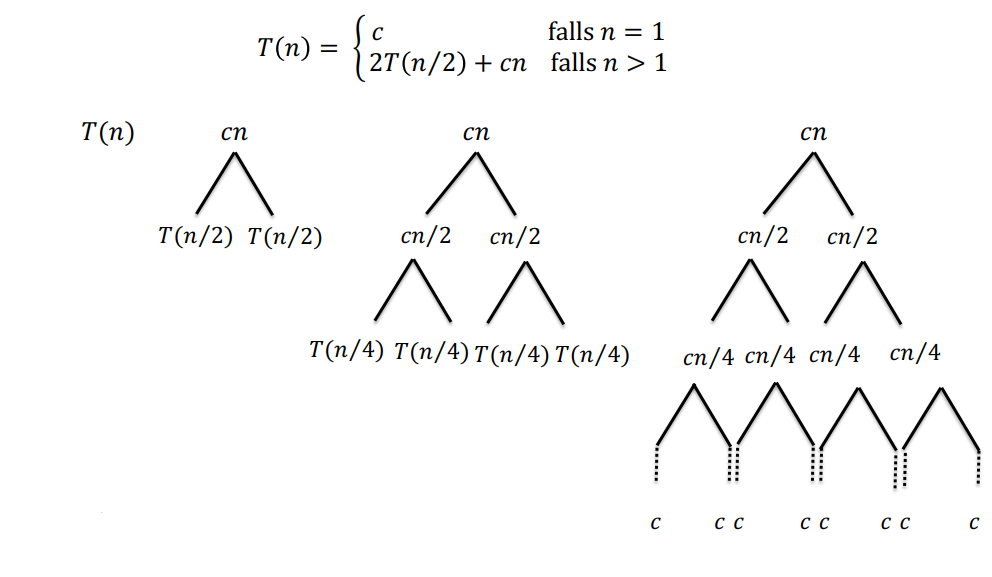
\includegraphics[width=12cm]{mergeSortBaum.PNG}
                        \item Verwenden der Konstante $c$ statt $\Theta(1)$
                        \item $cn$ stellt den Aufwand an der ersten Ebene dar 
                        \item Der addierte Aufwand jeder Stufe (aller Knoten) ist auch $cn$
                        \item Die Azahl der Ebenen lässt sich mithilfe von $lg(n) + 1$ bestimmen (2-er Logarithmus)
                        \item Damit ergibt sich für die Laufzeit: $cn \cdot lg(n)+cn$
                        \item Für $\lim_{n \rightarrow \infty}$ wird diese zu $n \cdot lg(n)$
                        \item Laufzeit beträgt damit $\Theta(n \cdot lg(n))$
                        \item Laufzeit von \texttt{MergaSort} ist in jedem Fall gleich
                    \end{itemize}
                
            \end{itemize}
    \end{itemize}

\subsection{Quicksort}
    \begin{itemize}
        \item \textbf{Idee}
            \begin{itemize}
                \item \textbf{Pivotelement}:
                    \begin{itemize}
                        \item[]
                            Wahl eines Pivotelement \texttt{x} aus dem Array
                    \end{itemize}

                \item \textbf{Divide:}
                    \begin{itemize}
                        \item[]
                            Zerlege den Array \texttt{A[p...r]} in zwei Teilarrays \texttt{A[p...q-1]} und \texttt{A[q+1...r]},
                            sodass jedes Element von \texttt{A[p...q-1]} kleiner oder gleich \texttt{A[q]} ist, welches
                            wiederum kleiner oder gleich jedem Element von \texttt{A[q+1...r]} ist. Berechnen Sie den Index \texttt{q}
                            als Teil vom \texttt{Partition} Algorithmus.
                    \end{itemize}

                \item \textbf{Conquer:}
                    \begin{itemize}
                        \item[]
                            Sortieren beider Teilarrays \texttt{A[p...q-1]} und \texttt{A[q+1...r]} durch rekursiven Aufruf von
                            Quicksort.
                    \end{itemize}
                
                \item \textbf{Combine:}
                    \begin{itemize}
                        \item[]
                            Da die Teilarrays bereits sortiert sind, ist keine weitere Arbeit nötig um diese zu vereinigen.
                            \texttt{A[p...r]} ist nun sortiert.
                    \end{itemize}
            \end{itemize}

        \item \textbf{Code}
            \begin{itemize}
                \item[]
                    \begin{minted}[autogobble,escapeinside=||]{c}
                    QUICKSORT(A,p,r)
                    IF p < r    // Überprüfung, ob Teilarray leer ist
                        q = PARTITION(A,p,r)
                        QUICKSORT(A,p,q-1)
                        QUICKSORT(A,q+1,r)
                    \end{minted}
                \item[]
                \item[]
                    \begin{minted}[autogobble,escapeinside=||]{c}
                    PARTITION(A,p,r)
                    x = A[r]    // Wahl des Pivotelements
                    i = p - 1   // Index i setzen
                    FOR j = p TO r - 1 // Auffüllen des Teilarrays mit Elementen
                        IF A[j] |$\leq$| x
                            i = i + 1
                            SWAP(A[i], A[j]) /
                    SWAP(A[i+1], A[r]) // Tausch des Pivotelements
                    RETURN i + 1 // Neuer Index des Pivotelements
                    \end{minted}
            \end{itemize}

        \item \textbf{Korrektheit von Quicksort}
            \begin{itemize}
                \item Schleifeninvariante:
                    \begin{itemize}
                        \item[]
                            Zu Beginn jeder Iteration der \texttt{for}-Schleife gilt für den Arrayindex $k$ folgendes:
                            \begin{enumerate}
                                \item Ist $p \leq k \leq i$, so gilt \texttt{A[k]} $\leq x$
                                \item Ist $i+1 \leq k \leq j -1$, so gilt \texttt{A[k]} $> x$
                                \item Ist $k = r$, so gilt \texttt{A[k]} $= x$ 
                            \end{enumerate}
                    \end{itemize}  
                
                \item Initialisierung:
                    \begin{itemize}
                        \item[]
                            Vor der ersten Iteration gilt $i = p - 1$ und $j = p$. Da es keine Werte zwischen $p$ und $j$
                            gibt und es auch keine Werte zwischen $i + 1$ und $j - 1$ gibt, sind die ersten beiden Eigenschaften
                            trivial erfüllt. Die Zuweisung in \texttt{x = A[r]} sorgt für die Erfüllung der dritten Eigenschaft.
                    \end{itemize}
                
                \item Fortsetzung:
                    \begin{itemize}
                        \item[]
                            Zwei mögliche Fälle durch \texttt{IF A[j] $\leq$ x}. Wenn \texttt{A[j] > x}, dann inkrementiert die 
                            Schleife nur den Index $j$. Dann gilt Bedingung 2 für \texttt{A[j-1]} und alle anderen Einträge
                            bleiben unverändert. Wenn \texttt{A[j] $\leq$ x}, dann wird Index $i$ inkrementiert und die 
                            Einträge \texttt{A[i]} und \texttt{A[j]} getauscht und schließlich der Index $j$ erhöht. Wegen
                            des Vertauschens gilt \texttt{A[i] $\leq$ x} und Bedingung 1 ist erfüllt. Analog gilt
                            \texttt{A[j-1] > x}, da das Element welches mit \texttt{A[j-1]} vertauscht wurde wegen der 
                            Invariante gerade größer als $x$ ist.
                    \end{itemize}

                \item Terminierung:
                    \begin{itemize}
                        \item[]
                            Bei der Terminierung gilt, dass $j = r$. Daher gilt, dass jeder Eintrag des Arrays zu einer der drei 
                            durch die Invariante beschriebenen Mengen gehört.
                    \end{itemize}
            \end{itemize}

        \item \textbf{Performanz von Quicksort}
            \begin{itemize}
                \item Abhängig von der \textbf{Balanciertheit} der Teilarrays 
                    \begin{itemize}
                        \item Definition Balanciert: ungefähr gleiche Anzahl an Elementen
                        \item Teilarrays balanciert: Laufzeit asymptotisch so schnell wie \texttt{MergeSort}
                        \item Teilarrays unbalanciert: Laufzeit kann so langsam wie \texttt{InsertionSort} laufen
                    \end{itemize}

                \item Zerlegung im \textbf{schlechtesten Fall}
                    \begin{itemize}
                        \item Partition zerlegt Problem in ein Teilproblem mit $n-1$ Elementen und eins mit $0$ Elementen
                        \item Unbalancierte Zerlegung zieht sich durch gesamte Rekursion
                        \item Zerlegung kostet $\Theta(n)$
                        \item Aufruf auf Feld der Größe 0: $T() = \Theta(1)$
                        \item Laufzeit (rekursiv):
                            \begin{itemize}
                                \item $T(n) = T(n-1) + T(0) + \Theta(n) = T(n-1) + \Theta(n)$
                                \item Insgesamt folgt: $T(n) = \Theta(n^2)$
                            \end{itemize}
                    \end{itemize}

                \item Zerlegung im \textbf{besten Fall}
                    \begin{itemize}
                        \item Problem wird so balanciert wie möglich zerlegt 
                        \item Zwei Teilprobleme mit maximaler Größe von $\frac{n}{2}$
                        \item Zerlegung kostet $\Theta(n)$
                        \item Laufzeit (rekursiv):
                            \begin{itemize}
                                \item $T(n) \leq 2T(\frac{n}{2}) + \Theta(n)$
                                \item Laufzeit beträgt: $O(n~lg(n))$
                            \end{itemize}
                        \item Solange die Aufteilung konstant bleibt, bleibt die Laufzeit $O(n~lg(n))$
                    \end{itemize}
                
            \end{itemize}
    \end{itemize}

\subsection{Laufzeitanalyse von rekursiven Algorithmen}
    \begin{itemize}
        \item \textbf{Analyse von Divide-And-Conquer Algorithmen}
            \begin{itemize}
                \item $T(n)$ ist Laufzeit eines Problems der Größe $n$
                \item Für kleines Problem benötigt die direkte Lösung eine konstante Zeit $\Theta(1)$
                \item Für sonstige $n$ gilt:
                    \begin{itemize}
                        \item Aufteilen eines Problems führt zu $a$ Teilproblemen
                        \item Jedes dieser Teilprobleme hat die Größe $\frac{1}{b}$ der Größe des ursprünglichen Problems
                        \item Lösen eines Teilproblems der Größe $\frac{n}{b}$: $T(\frac{n}{b})$
                        \item Lösen $a$ solcher Probleme: $a~T(\frac{n}{b})$
                        \item $D(n)$: Zeit um das Problem aufzuteilen (Divide)
                        \item $C(n)$: Zeit um Teillösungen zur Gesamtlösung zusammenzufügen (Combine)
                        \item[] \[
                                T(n) = \left.
                                    \begin{cases}
                                        \Theta(1) & \text{falls } n \leq c \\
                                        a~T(\frac{n}{b}) + D(n) + C(n) & \text{sonst}  \\
                                    \end{cases}
                                    \right \}
                                \]
                    \end{itemize}
            \end{itemize}

        \item \textbf{Subsitutionsmethode}
            \begin{itemize}
                \item Idee: Erraten einer Schranke und Nutzen von Induktion zum Beweis der Korrektheit
                \item Ablauf:
                    \begin{enumerate}
                        \item Rate die Form der Lösung (Scharfes Hinsehen oder kurze Eingaben ausprobieren/einsetzen)
                        \item Anwendung von vollständiger Induktion zum Finden der Konstanten und Beweis der Lösung
                    \end{enumerate}
                \item \textbf{Beispiel}
                    \begin{itemize}
                        \item Betrachten von \texttt{MergeSort}:
                            \begin{itemize}
                                \item $T(1) \leq c$
                                \item $T(n) \leq T(\left \lfloor \frac{n}{2} \right \rfloor) + T(\left \lceil \frac{n}{2} \right \rceil) + cn$
                            \end{itemize}

                        \item Ziel:
                            \begin{itemize}
                                \item[]
                                    Obere Abschätzung $T(n) \leq g(n)$ mit $g(n)$ ist eine Funktion, die durch eine 
                                    geschlossene Formel dargestellt werden kann.
                                \item[] 
                                    Wir \string"raten\string": $T(n) \leq 4cn~lg(n)$ und nehmen dies für alle $n' < n$ an und 
                                    zeigen es für $n$. 
                            \end{itemize}

                        \item Induktion:
                            \begin{itemize}
                                \item $lg$ steht hier für $log_2$
                                \item $n = 1$: $T(1) \leq c$
                                \item {\makebox[2cm][l]{$n = 2$: $T(2)$}}  $\leq T(1) + T(1) +2c$
                                \item[] {\makebox[2cm][l]{}} $\leq 4c \leq 8c$
                                \item[] {\makebox[1cm][l]{}} $T(2) = 4c * 2~lg(2) = 8c$
                            \end{itemize}

                        \item Hilfsbehauptungen:
                            \begin{itemize}
                                \item (1): $\left \lfloor \frac{n}{2} \right \rfloor + \left \lceil \frac{n}{2} \right \rceil = n$
                                \item (2): $\left \lfloor \frac{n}{2} \right \rfloor \leq \frac{n}{2} \leq \frac{2}{3}n$
                                \item (3): $log_c(\frac{a}{b}) = log_c(a) - log_c(b)$
                                \item (4): $log_c(a*b) = log_c(a) + log_c(b)$
                            \end{itemize}
                        \item Induktionsschritt:
                            \begin{itemize}
                                \item Annahme: $n > 2$ und sei Behauptung wahr für alle $n' < n$.
                                \item[]
                                    ${\makebox[1cm][l]{T(n)}}  \leq T(\left \lfloor \frac{n}{2} \right \rfloor) + T(\left \lceil \frac{n}{2} \right \rceil) + cn \\
                                    {\makebox[1cm][l]{}} \leq 4c \left \lfloor \frac{n}{2} \right \rfloor~ lg(\left \lfloor \frac{n}{2} \right \rfloor )
                                    + 4c \left \lceil \frac{n}{2} \right \rceil~ lg(\left \lceil \frac{n}{2} \right \rceil ) + cn \\
                                    {\makebox[1cm][l]{(HB)}} \leq 4c \cdot lg(\frac{2}{3}n) \cdot (\left \lfloor \frac{n}{2} \right \rfloor + \left \lceil \frac{n}{2} \right \rceil +cn \\
                                    {\makebox[1cm][l]{}} \leq 4c \cdot lg(\frac{2}{3}n) \cdot n + cn \\
                                    {\makebox[1cm][l]{(HB)}} \leq 4cn \cdot (lg(\frac{2}{3}) + lg(n)) + cn \\
                                    {\makebox[1cm][l]{}} = 4cn \cdot lg(n) + 4cn \cdot lg(\frac{2}{3}) \\
                                    {\makebox[1cm][l]{}} = 4cn \cdot lg(n) + cn (1+ 4 \cdot (lg(2) - lg(3))) \\
                                    {\makebox[1cm][l]{}} \leq 4cn \cdot lg(n) \\
                                    {\makebox[1cm][l]{}} \Rightarrow \Theta(n~lg(n))$
                            \end{itemize}
                    \end{itemize}
            \end{itemize}

        \item \textbf{Rekursionsbaum}
            \begin{itemize}
                \item Idee: Stellen das Ineinander-Einsetzen als Baum dar und Analyse der Kosten
                \item Ablauf:
                    \begin{enumerate}
                        \item Jeder Knoten stellt die Kosten eines Teilproblems dar 
                            \begin{itemize}
                                \item Die Wurzel stellt die zu analysierenden Kosten $T(n)$ dar 
                                \item Die Blätter stellen die Kosten der Basisfälle dar (z.B. $T(0)$)
                            \end{itemize}
                        \item Berechnen der Kosten innerhalb jeder Ebene des Baums
                        \item Die Gesamtkosten sind die Summe über die Kosten aller Ebenen
                    \end{enumerate}
                \item Rekursionsbaum ist nützlich um Lösung für Subsitutionsmethode zu erraten 
                \item \textbf{Beispiel:} $T(n) = 3T(\left \lfloor \frac{n}{4} \right \rfloor) + \Theta(n^2)$
                    \begin{itemize}
                        \item $\Rightarrow T(n) = 3T(\frac{n}{4}) + cn^2$ ($c>0$)
                        \item Je Abstieg verringert sich die Größe des Problems um den Faktor 4. 
                        \item Erreichen der Randbedingung ist vonnöten, die Frage ist wann dies geschieht.
                        \item Größe Teilproblem bei Level $i$: $\frac{n}{4^i}$
                        \item Erreichen Teilproblem der Größe 1, wenn $\frac{n}{4^i}=1$, d.h. wenn $i=log_4(n)$ \\
                            $\Rightarrow$ Baum hat also $log_4n + 1$ Ebenen
                        \item Kosten pro Ebene:
                            \begin{itemize}
                                \item Jede Ebene hat 3-mal soviele Knoten wie darüber liegende
                                \item Anzahl der Knoten in Tiefe $i$ ist $3^i$
                                \item Kosten $c(\frac{n}{4^i})^2~,~i=0...log_4n-1$
                                \item Anzahl $\cdot$ Kosten = $3^i \cdot c(\frac{n}{4^i})^2 = (\frac{3}{16})^i \cdot cn^2$
                            \end{itemize}
                        \item Unterste Ebene:
                            \begin{itemize}
                                \item $3^{log_4(n)} = n  {log_4(3)}$ Knoten
                                \item Jeder Knoten trägt $T(1)$ Kosten bei 
                                \item Kosten unten: $n^{log_4(3)} \cdot T(1) = \Theta(n^{log_4(3)})$
                            \end{itemize}
                        \item Addiere alle Kosten aller Ebenen:
                            \begin{itemize}
                                \item {\makebox[0.75cm][l]{$T(n)$}} $= cn^2 + \frac{3}{16}cn^2 + (\frac{3}{16})^2cn^2+...+ (\frac{3}{16})^{log_4n-1}cn^2 + \Theta(n^{log_4(3)})$
                                \item[] {\makebox[0.75cm][l]{}} $= \sum^{log_4n-1}_{i=0} (\frac{3}{16})^icn^2+ \Theta(n^{log_4^3})$
                                \item[] {\makebox[0.75cm][l]{}} $= \frac{(\frac{3}{16}^{log_4n})-1}{\frac{3}{16}-1} \cdot cn^2 + \Theta(n^{log_43})$ 
                                \item[] {\small (Verwendung der geometrischen Reihe)}
                                \item Verwendung einer unendlichen fallenden geometrischen Reihe als obere Schranke:
                                \item[] {\makebox[0.73cm][l]{$T(n)$}}  $= \sum^{log_4n-1}_{i=0} (\frac{3}{16})^i \cdot cn^2 + \Theta(n^{log_43})$
                                \item[] {\makebox[0.73cm][l]{}} $< \sum^{\infty}_{i=0} (\frac{3}{16})^i \cdot cn^2 + \Theta(n^{log_43})$
                                \item[] {\makebox[0.75cm][l]{}} $= \frac{1}{1-\frac{3}{16}} \cdot cn^2 + \Theta(n^{log_43})$ 
                                \item[] {\makebox[0.75cm][l]{}} $ = \frac{16}{13} \cdot cn^2 + Theta(n^{log_43}) = O(n^2)$
                            \end{itemize}
                        \item Jetzt \textbf{Subsitutionsmethode:}
                            \begin{itemize}
                                \item Zu zeigen: $\exists d > 0: T(n) \leq dn^2$
                                \item Induktionsanfang:
                                \item[] {\makebox[0.75cm][l]{$T(n)$}} $= 3 \cdot T(\left \lfloor \frac{1}{4} \right \rfloor) + c \cdot 1^2$
                                \item[] {\makebox[0.75cm][l]{}} $= 3 \cdot T(0) + c = c$
                                \item Induktionsschritt:
                                \item[] {\makebox[0.75cm][l]{$T(n)$}} $\leq 3 \cdot T(\left \lfloor \frac{n}{4} \right \rfloor) + cn^2$
                                \item[] {\makebox[0.75cm][l]{}} $\leq 3 \cdot d(\left \lfloor \frac{n}{4} \right \rfloor)^2+cn^2$
                                \item[] {\makebox[0.75cm][l]{}} $\leq 3d(\frac{n}{4})^2 + cn^2$
                                \item[] {\makebox[0.75cm][l]{}} $= \frac{3}{16}dn^2+cn^2$
                                \item[] {\makebox[0.75cm][l]{}} $\leq dn^2$, falls $d \geq \frac{16}{13}c$ 
                            \end{itemize}

                    \end{itemize}
            \end{itemize}

        \item \textbf{Mastertheorem}
            \begin{itemize}
                \item Idee:
                    \begin{itemize}
                        \item[] 
                            Seien $a \geq 1$ und $b > 1$ Konstanten. Sei $f(n)$ eine positive Funktion und $T(n)$ 
                            über den nichtnegativen ganzen Zahlen über die Rekursionsgleichung $T(n) = a~T(\frac{n}{b}) + f(n)$
                            defininiert, wobei wir $\frac{n}{b}$ so interpretieren, dass damit entweder $\left \lfloor \frac{n}{b} \right \rfloor$
                            oder $\left \lceil \frac{n}{b} \right \rceil$ gemeint ist. Dann besitzt $T(n)$ die folgenden asymptotischen Schranken
                            ($a$ und $b$ werden aus $f(n)$ gelesen):
                            \begin{enumerate}
                                \item Gilt $f(n) = O(n^{log_b (a - \epsilon)})$ für eine Konstante $\epsilon > 0$, dann $T(n) = \Theta(n^{log_b (a)})$
                                \item Gilt $f(n) = O(n^{log_b (a)})$, dann gilt $T(n) = \Theta(n^{log_b (a)} lg(n))$
                                \item Gilt $f(n) = \Omega(n^{log_b (a+\epsilon)})$ für eine Konstante $\epsilon > 0$ und $a~f(\frac{n}{b}) \leq c~f(n)$
                                      für eine \\ Konstante $c < 1$ und hinreichend großen $n$, dann ist $T(n) = \Theta(f(n))$
                            \end{enumerate}
                    \end{itemize}
                
                \item Erklärung:
                    \begin{itemize}
                        \item In jedem der 3 Fälle wird die Funktion $f(n)$ mit $n^{log_b(a)}$ verglichen
                            \begin{enumerate}
                                \item Wenn $f(n)$ polynomial kleiner ist als $n^{log_b(a)}$, dann $T(n) = \Theta(n^{log_b(a)})$
                                \item Wenn $f(n)$ und $n^{log_b(a)}$ die gleiche Größe haben, gilt $T(n) = \Theta(n^{log_b (a)} lg(n))$
                                \item Wenn $f(n)$ polynomial größer als $n^{log_b(a)}$ und $a~f(\frac{n}{b}) \leq c~f(n)$ erfüllt, dann $T(n) = \Theta(f(n))$
                            \end{enumerate}
                        \item (polynomial größer/kleiner: um Faktor $n^\epsilon$ asymptotisch größer/kleiner)
                    \end{itemize}

                \item Nicht abgedeckte Fälle:
                    \begin{itemize}
                        \item Wenn einer dieser Fälle eintritt, kann das Mastertheorem nicht angewendet werden
                            \begin{enumerate}
                                \item Wenn $f(n)$ kleiner ist als $n^{log_b(a)}$, aber nicht polynomial kleiner
                                \item Wenn $f(n)$ größer ist als $n^{log_b(a)}$, aber nicht polynomial größer
                                \item Regularitätsbedingung $a~f(\frac{n}{b}) \leq c~f(n)$ wird nicht erfüllt
                                \item $a$ oder $b$ sind nicht konstant (z.B. $a=2^n$)
                            \end{enumerate}
                    \end{itemize}

                \item \textbf{Beispiel:}
                    \begin{itemize}
                        \item $T(n) = 9T(\frac{n}{3}) + n$
                            \begin{itemize}
                                \item $a=9, b=3, f(n)=n$
                                \item $log_b(a) = log_3(9) = 2$
                                \item {\makebox[1.5cm][l]{$f(n) = n$}} $= O(n^{log_b(a-\epsilon)})$
                                \item[] {\makebox[1.5cm][l]{}} $= O(n^{2-\epsilon})$
                                \item Ist diese Gleichung für ein $\epsilon > 0$ erfüllt? $\Rightarrow$ $\epsilon = 1$
                                \item \textbf{1. Fall} $\Rightarrow$ $T(n) = \Theta(n^2)$ 
                            \end{itemize}

                        \item $T(n) = T(\frac{2n}{3}) + 1$
                            \begin{itemize}
                                \item $a=1, b= \frac{3}{2}, f(n) = 1$
                                \item $log_{\frac{3}{2}} 1 = 0$
                                \item {\makebox[1.5cm][l]{$f(n) = 1$}} $= O(n^{log_b(a)})$
                                \item[] {\makebox[1.5cm][l]{}} $= O(n^0)$
                                \item[] {\makebox[1.5cm][l]{}} $= O(1)$
                                \item \textbf{2.Fall} $\Rightarrow$ $T(n) = \Theta(1 * lg(n)) = \Theta(lg(n))$   
                            \end{itemize}

                        \item $T(n) = 3(T\frac{n}{4}) + n~lg(n)$
                            \begin{itemize}
                                \item $a=3,b=4,f(n)= n~lg(n)$
                                \item $n^{log_b(a)} = n^{log_4(3)} \leq n^{0.793}$
                                \item $\epsilon = 0.1$ im Folgenden
                                \item $f(n) = n~lg(n) \geq n \geq n^{0.793 + 0.1} \geq n^{0.793}$ 
                                \item \textbf{3.Fall} $\Rightarrow$ $f(n) = \Omega(n^{log_b(a+0.1)})$
                                \item $a f(\frac{n}{b}) = 3f(\frac{n}{4}) = 3(\frac{n}{4})~lg(\frac{n}{4}) \leq \frac{3}{4} n~lg(n)$
                                \item Damit ist auch die Randbedingung erfüllt und $T(n) = \Theta(n~lg(n))$
                                
                            \end{itemize}
                    \end{itemize}
            \end{itemize}

    \end{itemize}

\pagebreak

\section{Grundlegende Datenstrukturen}
\subsection{Stacks}
    \begin{itemize}
        \item \textbf{Abstrakter Datentyp Stack}
            \begin{itemize}
                \item \texttt{new S()}
                    \begin{itemize}
                        \item Erzeugt neuen (leeren) Stack
                    \end{itemize}
                \item \texttt{s.isEmpty()}
                    \begin{itemize}
                        \item Gibt an, ob Stack \texttt{s} leer ist
                    \end{itemize}
                \item \texttt{s.pop()}
                    \begin{itemize}
                        \item Gibt oberstes Element vom Stack \texttt{s} zurück und löscht es vom Stack 
                        \item Gibt Fehlermeldung aus, falls der Stack leer ist 
                    \end{itemize}
                \item \texttt{s.push(k)}
                    \begin{itemize}
                        \item Schreibt \texttt{k} als neues oberstes Element auf Stack \texttt{s}
                    \end{itemize}
                \item Abstrakter Aufbau:
                    \begin{itemize}
                        \item \textbf{LIFO}-Prinzip - Last in, First out 
                        \item[] 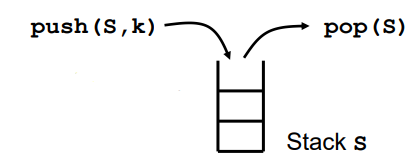
\includegraphics[width=6cm]{stack1.PNG}
                    \end{itemize}
            \end{itemize}

        \item \textbf{Beispiel Bitcoin}
        \item[] 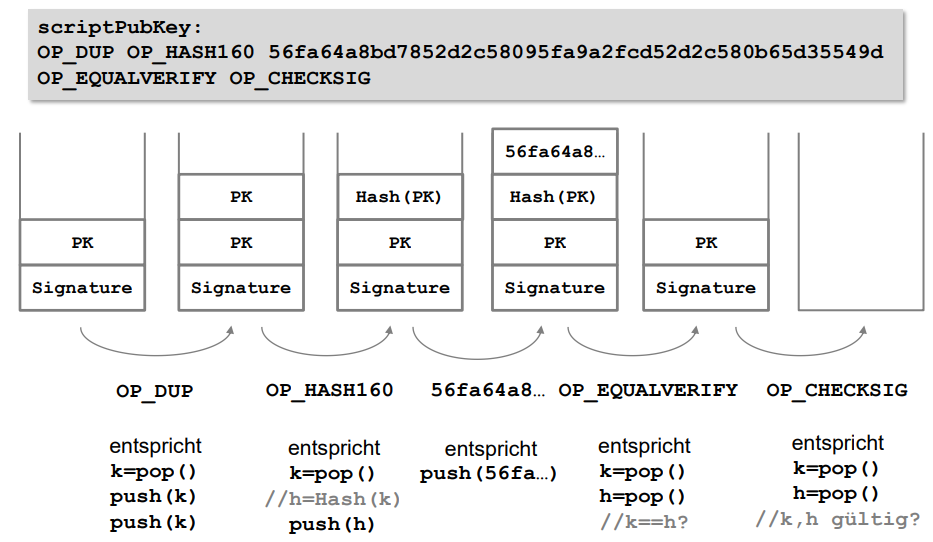
\includegraphics[width=15cm]{stackBitcoin.PNG}
        
        \item \textbf{Stacks als Array}
            \begin{itemize}
                \item[] 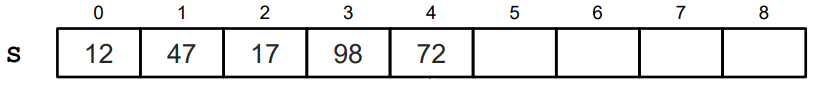
\includegraphics[width=12cm]{stackArray.PNG}  
                \item \texttt{s.top} zeigt immer auf oberstes Element 
                \item \texttt{pop()} führt dazu, dass \texttt{s.Top} sich eins nach links bewegt
                \item \texttt{push(k)} führt dazu, dass \texttt{s.Top} sich eins nach rechts bewegt
            \end{itemize}

        \item \textbf{Stacks als Array - Methoden, falls maximale Größe bekannt}
        \item[] 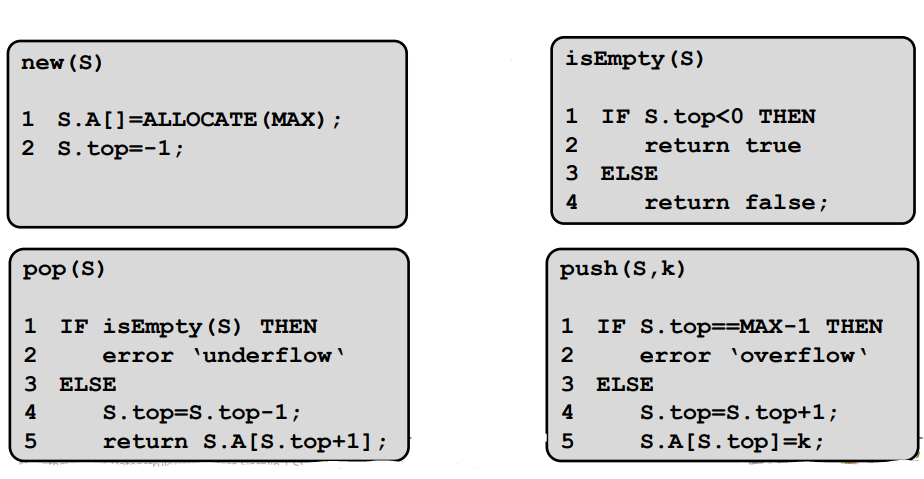
\includegraphics[width=12cm]{arrayMethods1}

        \item \textbf{Stacks mit variabler Größe - Einfach}
            \begin{itemize}
                \item Falls \texttt{push(k)} bei vollem Array $\Rightarrow$ Vergößerung des Arrays
                \item Erzeugen eines neuen Arrays mit Länge + 1 und Umkopieren aller Elemente
                \item Durchschnittlich $\Omega(n)$ Kopierschritte pro \texttt{push}-Befehl
            \end{itemize}

        \item \textbf{Stacks mit variabler Größe - Verbesserung}
            \begin{itemize}
                \item Idee: 
                    \begin{itemize}
                        \item Wenn Grenze erreicht, Verdopplung des Speichers und Kopieren der Elemente
                        \item Falls weniger als ein Viertel belegt, schrumpfe das Array wieder 
                    \end{itemize}
                \item Methoden:
                \item[] \texttt{RESIZE(A,m)} reserviert neuen Speicher der Grö\ss e \texttt{m} und kopiert \texttt{A} um
                \item[] 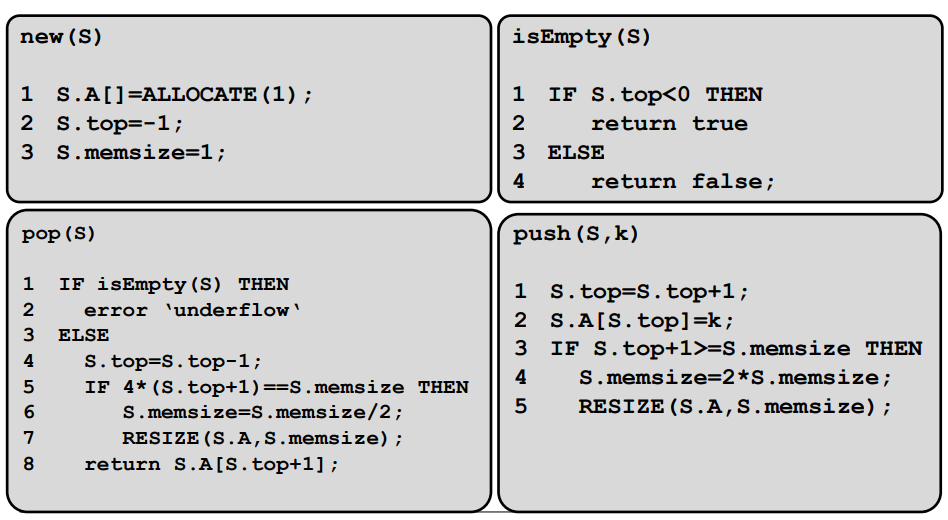
\includegraphics[width=12cm]{stacksArray2.PNG}

                \item Im Durchschnitt für jeder der mindestens \texttt{n} Befehle $\Theta(1)$ Umkopierschritte
                
            \end{itemize}
    \end{itemize}

\subsection{Verkettete Listen}
    \begin{itemize}
        \item \textbf{Aufbau}
            \begin{itemize}
                \item[] 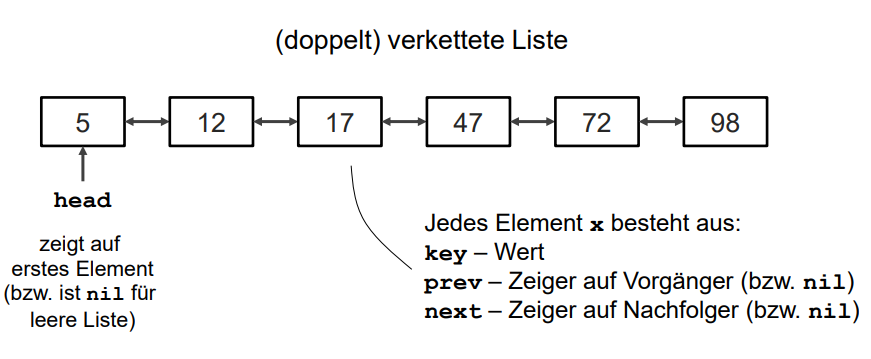
\includegraphics[width=12cm]{linkedList1.PNG}
            \end{itemize}
        
        \item \textbf{Verkettete Listen durch Arrays}
            \begin{itemize}
                \item[] Entspricht doppelter Verkettung zwischen 45 und 12
                \item[] 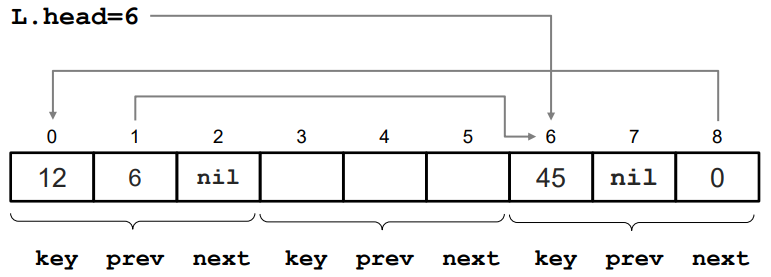
\includegraphics[width=12cm]{linkedList2.PNG}
            \end{itemize}

        \item \textbf{Elementare Operationen auf Listen}
            \begin{itemize}
                \item Suche nach Element
                    \begin{itemize}
                        \item Laufzeit beträgt im Worst Case $\Theta(n)$
                        \item[] $\Rightarrow$ Keine Überprüfung, ob Wert bereits in Liste, sonst $\Theta(n)$
                        \item Code:
                        \item[] 
                            \begin{minted}[autogobble]{c}
                            search(L,k)    // Returns pointer to k in L (or nil)
                            current = L.head;
                            WHILE current != nil AND current.key != k DO 
                                current = current.next;
                            return current;
                            \end{minted}
                    \end{itemize}

                \item Einfügen eines Elements am Kopf der Liste 
                    \begin{itemize}
                        \item Laufzeit beträgt $\Theta(1)$, da Einfügen am Kopf 
                        \item Code:
                        \item[] 
                            \begin{minted}[autogobble]{c}
                            insert(L,x)
                            x.next = l.head;
                            x.prev = nil;
                            IF L.head != nil THEN 
                                L.head.prev = x;
                            L.head = x;
                            \end{minted}
                    \end{itemize}

                \item Löschen eines Elements aus Liste
                    \begin{itemize}
                        \item Laufzeit beträgt $\Theta(1)$, da hier Pointer auf Objekt gegeben
                        \item[] Löschen eines Wertes $k$ mithilfe von Suche beträgt $\Omega(n)$
                        \item Code:
                        \item[]
                            \begin{minted}[autogobble]{c}
                            delete (L,x)
                            IF x.prev != nil THEN
                                x.prev.next = x.next
                            ELSE 
                                L.head = x.next;
                            IF x.next != nil THEN
                                x.next.prev = x.prev;
                            \end{minted} 
                    \end{itemize}
            \end{itemize}

        \item \textbf{Vereinfachung per Wächter/Sentinels}
            \begin{itemize}
                \item Ziel ist die Eliminierung der Spezialfälle für Listenanfang/-ende 
                \item[] 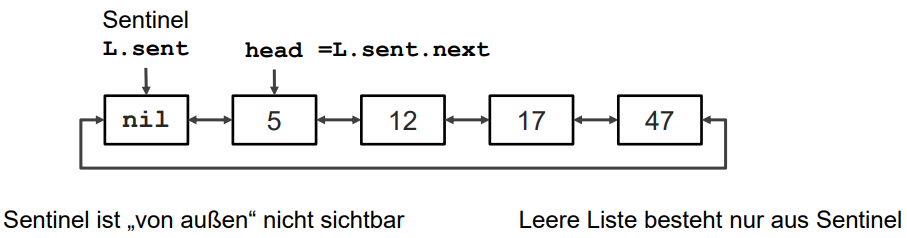
\includegraphics[width=12cm]{linkedListSentinel.PNG}
                \item Löschen mit Sentinels:
                \item[]
                    \begin{minted}[autogobble]{c}
                    deleteSent(L,x)
                    x.prev.next = x.next;
                    x.next.prev = x.prev;
                    \end{minted}
            \end{itemize}
    \end{itemize}

\subsection{Queues}
    \begin{itemize}
        \item \textbf{Abstrakter Datentyp Queue}
            \begin{itemize}
                \item \texttt{new Q()}
                    \begin{itemize}
                        \item Erzeuge neue (leere) Queue
                    \end{itemize}
                
                \item \texttt{q.isEmpty()}
                    \begin{itemize}
                        \item Gibt an, ob Queue \texttt{q} leer ist 
                    \end{itemize}
                
                \item \texttt{q.dequeue()}
                    \begin{itemize}
                        \item Gibt vorderstes Element aus \texttt{q} zurück und löscht es auf Queue 
                        \item Fehlermeldung, falls Queue leer ist 
                    \end{itemize}
                
                \item \texttt{q.enqueue(k)} 
                    \begin{itemize}
                        \item Schreibt \texttt{k} als neues hinterstes Element auf \texttt{q}
                        \item Fehlermeldung, falls Queue voll ist 
                    \end{itemize}
                
                \item Abstrakter Aufbau:
                    \begin{itemize}
                        \item \textbf{FIFO}-Prinzip / First in, First out 
                        \item[] 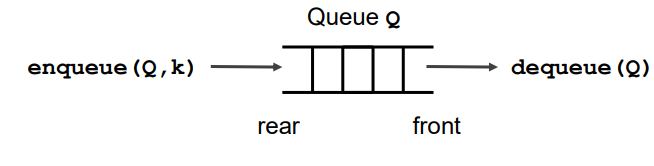
\includegraphics[width=8cm]{queueAbstract}
                    \end{itemize}
            \end{itemize}

        \item \textbf{Queues als (virtuelles) zyklisches Array}
            \begin{itemize}
                \item[] Bekannt: Maximale Elemente gleichzeitig in Queue
                \item[] 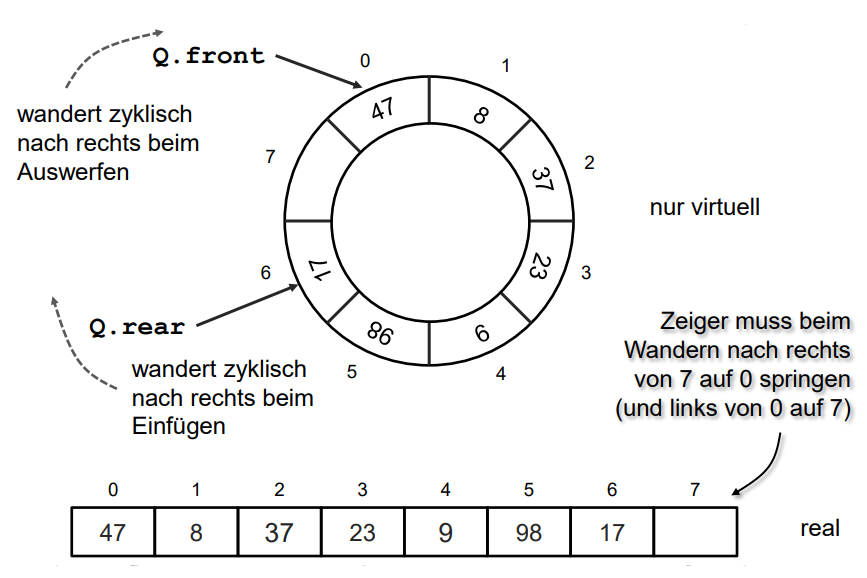
\includegraphics[width=12cm]{queueZyklisch.PNG} 
                \item[] 
                \item Problem, falls \texttt{Q.rear} und \texttt{Q.front} auf selbes Element zeigen 
                    \begin{itemize}
                        \item Speichere Information, ob Schlange leer oder voll, in boolean \texttt{empty}
                        \item Alternativ: Reserviere ein Element des Arrays als Abstandshalter
                    \end{itemize}
                
                \item Methoden für zyklisches Array
                \item[] 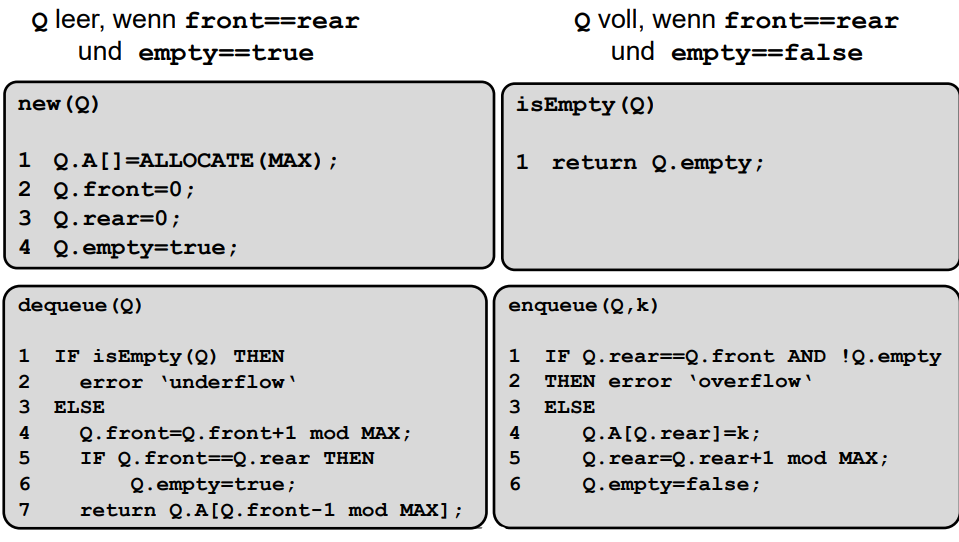
\includegraphics[width=12cm]{queueZyklischM.PNG}
            \end{itemize}

        \item \textbf{Queues durch einfach verkettete Listen}
            \begin{itemize}
                \item[] 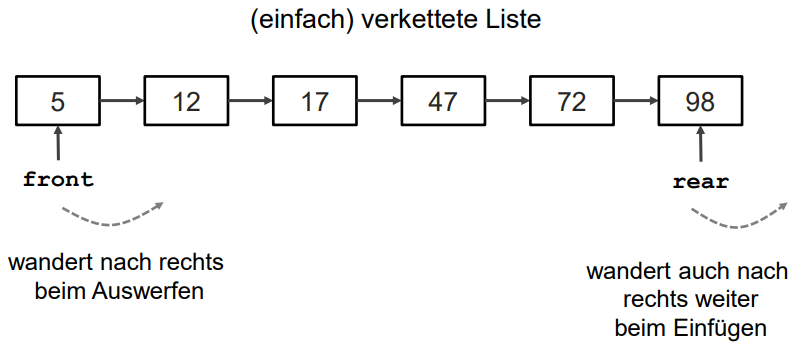
\includegraphics[width=12cm]{queuesListe1.PNG}
                \item[] Methoden:
                \item[] 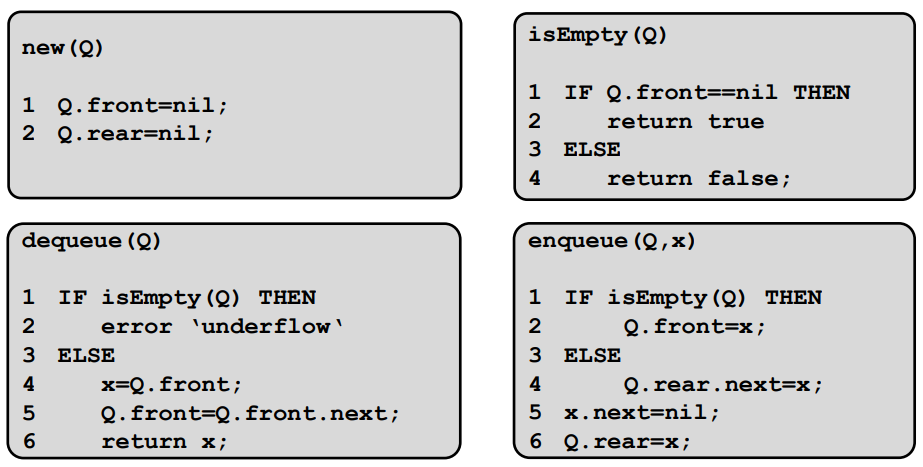
\includegraphics[width=12cm]{queuesListe2.PNG} 
            \end{itemize}

        \item \textbf{Laufzeit}
            \begin{itemize}
                \item Enqueue: $\Theta(1)$
                \item Dequeue: $\Theta(1)$
            \end{itemize}
    \end{itemize}

\pagebreak

\subsection{Binäre Bäume}
    \begin{itemize}
        \item \textbf{Bäume durch verkettete Listen}
            \begin{itemize}
                \item[] \includegraphics[width=12cm]{binäreBaumeListe.PNG}
                \item[] Bäume sind \string"azyklisch\string" (Keine "rückführende Spur")   
            \end{itemize}

        \item \textbf{Darstellung als (ungerichteter) Graph}
            \begin{itemize}
                \item[]
                    \begin{minipage}[t]{0.45\textwidth}
                        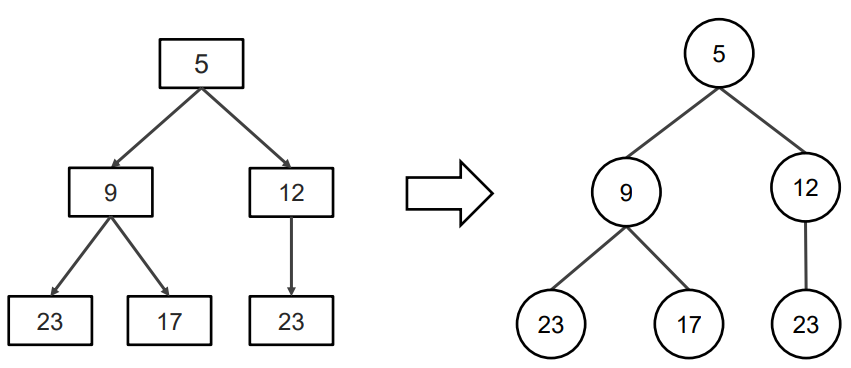
\includegraphics[width=7cm]{baumGraph1.PNG}
                    \end{minipage}
                    \begin{minipage}[t]{0.45\textwidth}
                        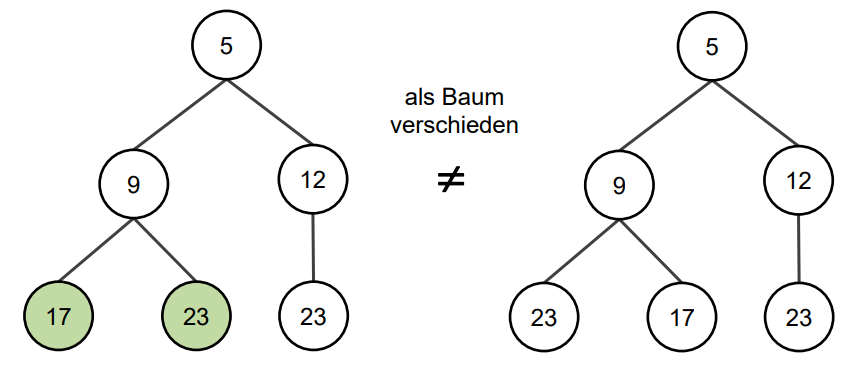
\includegraphics[width=7cm]{baumGraph2.PNG}
                    \end{minipage}
            \end{itemize}
        
            \item \textbf{Allgemeine Begrifflichkeiten}
                \begin{itemize}
                    \item[]
                        \begin{minipage}[t]{0.45\textwidth}
                            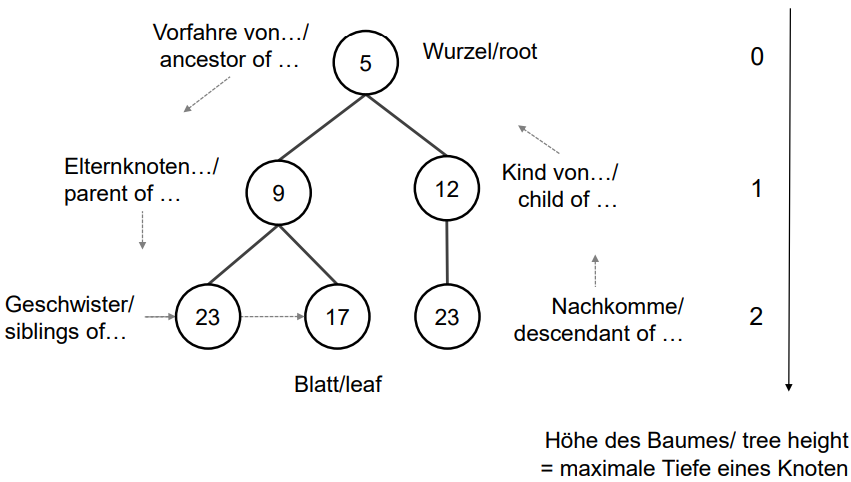
\includegraphics[width=8cm]{baumBegriffe1.PNG}
                        \end{minipage}
                        \begin{minipage}[t]{0.45\textwidth}
                            \vspace{-3.5cm}
                            \begin{itemize}
                                \item Blatt: Knoten ohne Nachfolger
                                \item Nachkomme von x: \\
                                        Erreichbar durch Pfad ausgehend von x
                            \end{itemize}
                        \end{minipage}
                \end{itemize}

            \item \textbf{Begrifflichkeiten Binärbaum}
                \begin{itemize}
                    \item[]
                        \begin{minipage}[t]{0.45\textwidth}
                            \includegraphics[width=8cm]{binärbaumBegriffe}
                        \end{minipage}
                        \begin{minipage}[t]{0.45\textwidth}
                            \vspace{-4.5cm}
                            \begin{itemize}
                                \item Jeder Knoten hat maximal zwei Kinder \\
                                        \texttt{left=child[0]} und \texttt{right=child[1]}
                                \item Ausgangsgrad jedes Knoten ist $\leq 2$
                                \item Höhe leerer Baum per Konvention $-1$
                                \item Hohe (nicht-leerer) Baum: \\
                                        max\{Höhe aller Teilbäume der Wurzel\} + 1
                                \item Halbblatt: Knoten mit nur einem Kind
                            \end{itemize}
                        \end{minipage}
                \end{itemize}

                \pagebreak

            \item \textbf{Traversieren von Bäumen}
                \begin{itemize}
                    \item Darstellung eines Baumes mithilfe einer Liste der Werte aller Knoten
                    \item Laufzeit bei $n$ Knoten: $T(n) = O(n)$
                    \item Nutzung der Preorder für das Kopieren von Bäumen 
                        \begin{enumerate}
                            \item Preorder betrachtet Knoten und legt Kopie an
                            \item Preorder geht dann in Teilbäume und kopiert diese
                        \end{enumerate}
                    \item Nutzung der Postorder für das Löschen von Bäumen
                        \begin{enumerate}
                            \item Postorder geht zuerst in Teilbäume und löscht diese 
                            \item Betrachten des Knoten erst danach und dann Löschung dieses
                        \end{enumerate}
                    \item[]
                    \item[]
                        \begin{minipage}[t]{0.4\textwidth}
                            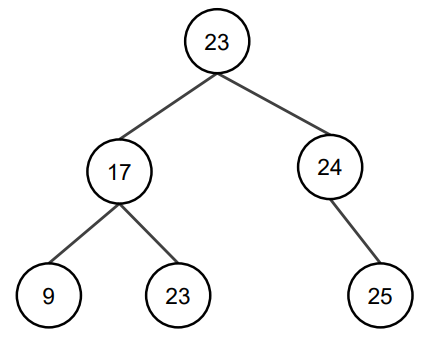
\includegraphics[width=6cm]{inorder1}           
                        \end{minipage}
                        \begin{minipage}[t]{0.5\textwidth}
                            \vspace{-4.75cm}
                            \begin{itemize}
                                \item[] 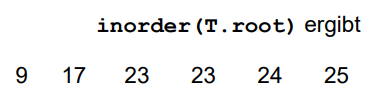
\includegraphics[width=6cm]{inorder2}
                                \item[] 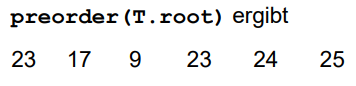
\includegraphics[width=6cm]{preorder1}
                                \item[] 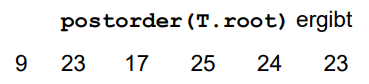
\includegraphics[width=6cm]{postorder1}
                            \end{itemize}
                        \end{minipage}
                    \item[]
                    \item[] \textbf{Code:} \\
                        \begin{minipage}[t]{0.3\textwidth}
                            \begin{minted}[autogobble]{c}
                            inorder(x)
                            IF x != nil THEN 
                                inorder(x.left);
                                print x.key;
                                inorder(x.right);
                            \end{minted}
                        \end{minipage}
                        \begin{minipage}[t]{0.3\textwidth}
                            \begin{minted}[autogobble]{c}
                            preorder(x)
                            IF x != nil THEN
                            print x.key;
                            preorder(x.left);
                            preorder(x.right);
                            \end{minted}
                        \end{minipage}
                        \begin{minipage}[t]{0.3\textwidth}
                            \begin{minted}[autogobble]{c}
                            postorder(x)
                            IF x != nil THEN
                                postorder(x.left);
                                postorder(x.right);
                                print x.key;
                            \end{minted}
                        \end{minipage}
                \end{itemize}

            \item \textbf{Eindeutige Bestimmbarkeit von Bäumen}
                \begin{itemize}
                    \item Nur In-,Pre-,Postorder reichen nicht zur eindeutigen Bestimmbarkeit von Bäumen
                    \item[] $\Rightarrow$ Preorder/Postorder $+$ Inorder $+$ eindeutige Werte sind notwendig
                    \item[] 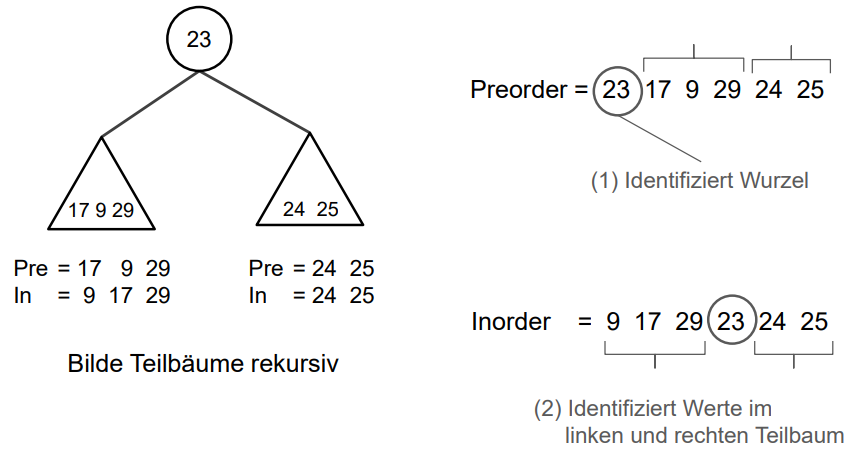
\includegraphics[width=12cm]{bestimmbarkeitBaum.PNG} 
                \end{itemize}

                \pagebreak

            \item \textbf{Abstrakter Datentyp Baum}
                \begin{itemize}
                    \item Abstrakter Aufbau:
                        \begin{itemize}
                            \item \texttt{new T()}
                                \begin{itemize}
                                    \item Erzeugt neuen Baum namens \texttt{t}
                                \end{itemize}

                            \item \texttt{t.search(k)}
                                \begin{itemize}
                                    \item Gibt Element \texttt{x} in Baum \texttt{t} mit \texttt{x.key == k} zurück
                                \end{itemize}
                            
                            \item \texttt{t.insert(k)}
                                \begin{itemize}
                                    \item Fügt Element \texttt{x} in Baum \texttt{t} hinzu
                                \end{itemize}
                            
                            \item \texttt{t.delete(x)}
                                \begin{itemize}
                                    \item Löscht \texttt{x} aus Baum \texttt{t}
                                \end{itemize}
                        \end{itemize}

                    \item Suche nach Elementen
                        \begin{itemize}
                            \item Laufzeit = $\Theta(n)$ (Jeder Knoten maximal einmal, jeder Knoten im schlechtesten Fall)
                            \item Starte mit \texttt{search(T.root,k)}
                            \item Code:
                            \item[]
                                \begin{minted}[autogobble]{c}
                                search(x,k)
                                IF x == nil THEN return nil;
                                IF x.key == k THEN return x;
                                y = search(x.left,k);
                                IF y != nil THEN return y;
                                return search(x.right,k);
                                \end{minted}
                        \end{itemize}

                    \item Einfügen von Elementen
                        \begin{itemize}
                            \item Laufzeit = $\Theta(1)$ 
                            \item Hier wird als Wurzel eingefügt (Achtung: Erzeugt linkslastigen Baum)
                            \item Code:
                            \item[]
                                \begin{minted}[autogobble]{c}
                                insert(T,x) // x.parent == x.left == x.right == nil;
                                IF T.root != nil THEN 
                                    T.root.parent = x;
                                    x.left = T.root;
                                T.root = x;
                                \end{minted}
                        \end{itemize}

                    \item Löschen von Elementen
                        \begin{itemize}
                            \item Laufzeit = $\Theta(h)$ (Höhe des Baumes, $h=n$ möglich)
                            \item Hier: Ersetze $x$ durch Halbblatt ganz rechts
                            \item[] \includegraphics[width=12cm]{löschenBaum.PNG}
                            \item \texttt{Connect}-Algorithmus:
                            \item[]
                                \begin{minipage}[t]{0.35\textwidth}
                                    \includegraphics[width=5cm]{löschenBaumConnect.PNG}
                                \end{minipage}
                                \begin{minipage}[t]{0.45\textwidth}
                                    \vspace{-7cm}
                                    \begin{itemize}
                                        \item Laufzeit = $\Theta(1)$
                                        \item[]
                                            \begin{minted}[autogobble]{c}
                                            connect(T,y,w) // Connects w to y.parent
                                            v = y.parent;
                                            IF y != T.root THEN 
                                                IF y == v.right THEN 
                                                    v.right = w;
                                                ELSE 
                                                    v.left = w;
                                            
                                            ELSE 
                                                T.root = w;
                                            
                                            IF w != nil THEN 
                                                w.parent = v;
                                            \end{minted}
                                    \end{itemize}
                                \end{minipage}

                            \item \texttt{Delete}-Algorithmus:
                            \item[]
                                \begin{minipage}{0.4\textwidth}
                                    \includegraphics[width=6cm]{löschenBaumDelete.PNG}
                                \end{minipage}
                                \begin{minipage}{0.5\textwidth}
                                    \begin{itemize}
                                        \item[]
                                            \begin{minted}[autogobble]{c}
                                            delete(T,x) // assumes x in T
                                            y = T.root;
                                            WHILE y.right != nil DO 
                                                y = y.right;
                                            
                                            connect(T,y,y.left);

                                            if x != y THEN
                                                y.left = x.left;
                                                IF x.left != nil THEN
                                                    x.left.parent = y;
                                                y.right = x.right;
                                                IF x.right != nil THEN
                                                    x.right.parent = y;
                                                connect(T,x,y);
                                            \end{minted}
                                    \end{itemize}
                                \end{minipage}
                        \end{itemize}
                \end{itemize}
    \end{itemize}

\subsection{Binäre Suchbäume}
    \begin{itemize}
        \item \textbf{Definition}
            \begin{itemize}
                \item Totale Ordnung auf den Werten 
                \item Für alle Knoten $z$ gilt:
                \item[] Wenn $x$ Knoten im linken Teilbaum von $z$, dann \texttt{x.key $\leq$ z.key}
                \item[] Wenn $y$ Knoten im rechten Teilbaum von $z$, dann \texttt{y.key $\geq$ z.key} 
                \item Preorder/Postorder + eindeutige Werte $\Rightarrow$ Eindeutige Identifizierung 
            \end{itemize}
        
        \item \textbf{Suchen im Binären Suchbaum}
            \begin{itemize}
                \item[]
                    \begin{minipage}{0.4\textwidth}
                        \includegraphics[width=8cm]{binärerSuchbaumSuche.PNG}
                    \end{minipage}
                    \begin{minipage}{0.5\textwidth}
                        \begin{itemize}
                            \item Laufzeit $= O(h)$ (Höhe)
                            \item Code:
                            \item[]
                                \begin{minted}[autogobble]{c}
                                search(x,k) // 1. Aufruf x = root
                                IF x == nil OR x.key == k THEN
                                    return x;
                                IF x.key > k THEN
                                    return search(x.left,k);
                                ELSE
                                    return search(x.right,k);
                                \end{minted}
                            \item Iterativer Code:
                            \item[]
                                \begin{minted}[autogobble]{c}
                                iterative-search(x,k)
                                WHILE x != nil AND x.key != k DO
                                    IF x.key > k THEN
                                        x = x.left;
                                    ELSE
                                        x = x.right;
                                return x;
                                \end{minted}
                        \end{itemize}
                    \end{minipage}
            \end{itemize}

        \item \textbf{Einfügen im Binary Search Tree}
            \begin{itemize}
                \item[]
                    \begin{minipage}{0.4\textwidth}
                        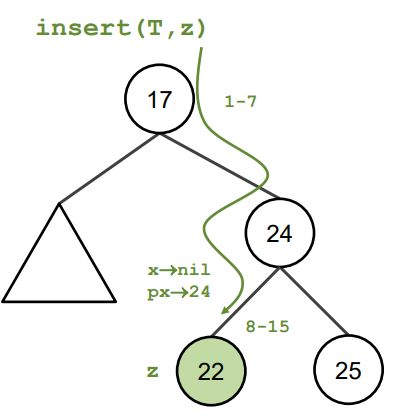
\includegraphics[width=8cm]{binärerSuchbaumEinfügen.PNG}
                    \end{minipage}
                    \begin{minipage}{0.5\textwidth}
                        \begin{itemize}
                            \item Laufzeit = $O(h)$
                            \item Aufwendiger, da Ordnung erhalten werden muss
                            \item Code:
                            \item[]
                                \begin{minted}[autogobble]{c}
                                insert (T,z) // z.left == z.right == nil;
                                x = T.root;
                                px = nil;
                                WHILE x != nil DO
                                    px = x;
                                    IF x.key > z.key THEN
                                        x = x.left;
                                    ELSE 
                                        x = x.right;
                                z.parent = px;
                                IF px == nil THEN
                                    T.root = z;
                                ELSE 
                                    IF px.key > z.key THEN
                                        px.left = z;
                                    ELSE 
                                        px.right = z;
                                \end{minted}
                        \end{itemize}
                    \end{minipage}
            \end{itemize}

\pagebreak

        \item \textbf{Löschen im BST}
            \begin{itemize}
                \item Verschiedene Fälle:
                    \begin{itemize}
                        \item[] 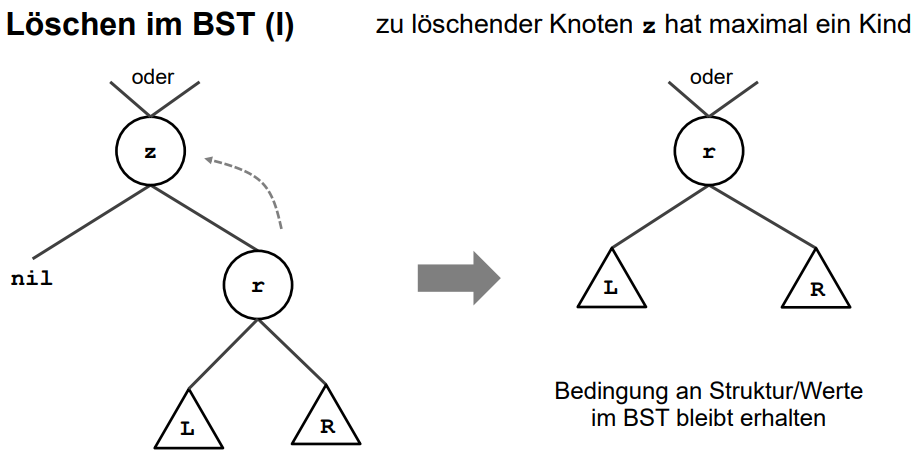
\includegraphics[width=9cm]{binärerSuchbaumLöschen1.PNG}
                        \item[] 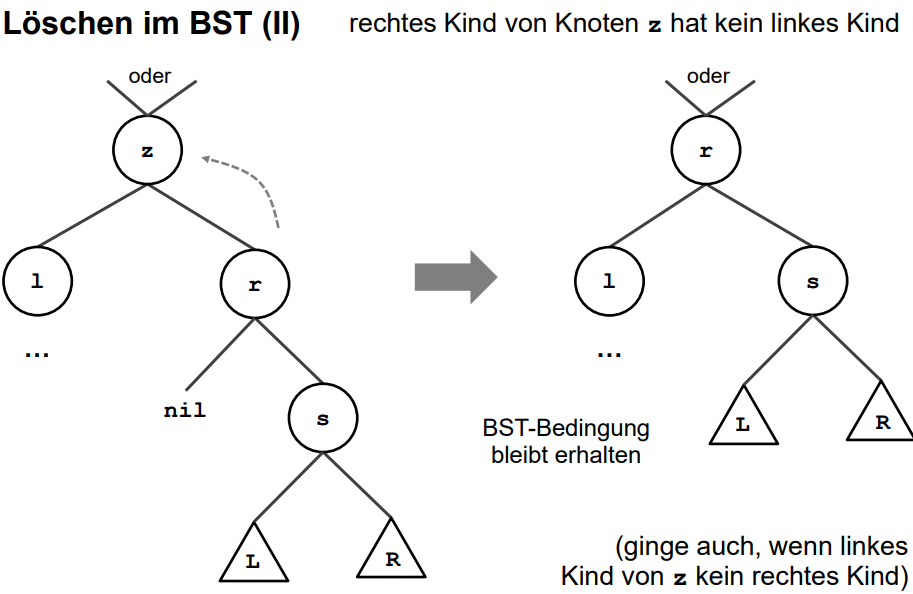
\includegraphics[width=9cm]{binärerSuchbaumLöschen2.PNG} 
                        \item[] 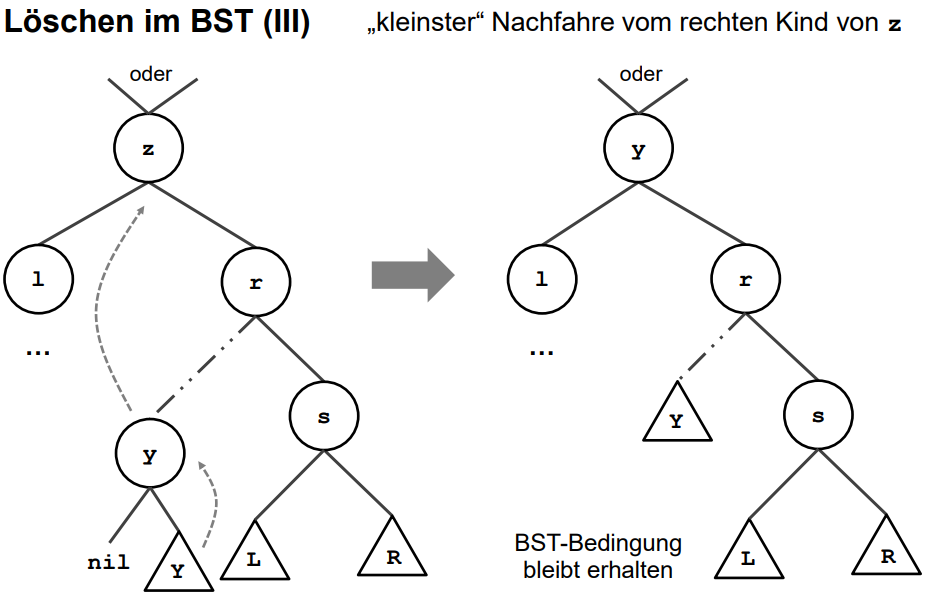
\includegraphics[width=9cm]{binärerSuchbaumLöschen3.PNG} 
                    \end{itemize}

                \item Code (Transplantation)
                \item[]
                    \begin{minipage}{0.45\textwidth}
                            \begin{minted}[autogobble]{c}
                            // Hängt Teilbaum v an Parent von u
                            transplant(T,u,v) 
                            IF u.parent == nil THEN
                                T.root = v;
                            ELSE
                                IF u == u.parent.left THEN
                                    u.parent.left = v;
                                ELSE 
                                    u.parent.right = v;
                            IF v != nil THEN
                                v.parent = u.parent;
                            \end{minted}
                    \end{minipage}
                    \begin{minipage}{0.45\textwidth}
                        \begin{minted}[autogobble]{c}
                        delete(T,z)
                        IF z.left == nil THEN
                            transplant(T,z,z.left)
                        ELSE
                            IF z.right == nil THEN
                                transplant(T,z,z,left)
                            ELSE
                                y = z.right;
                                WHILE y.left != nil DO y = y.left;
                                IF y.parent != z THEN
                                    transplant(T,y,y.right)
                                    y.right = z.right;
                                    y.right.parent = y;
                                transplant(T,z,y)
                                y.left = z.left;
                                y.left.parent = y;
                        \end{minted}
                    \end{minipage}
                \item Laufzeit = $O(h)$
                \item Laufzeit ist damit besser, wenn viele Suchoperationen und $h$ klein relativ zu $n$
            \end{itemize}

        \item \textbf{Höhe eines BST}
            \begin{itemize}
                \item Best Case:
                    \begin{itemize}
                        \item Vollständiger Baum (Alle Blätter gleiche Tiefe)
                        \item $h = O(log_2 n)$
                        \item Laufzeit = $O(log_2 n)$
                    \end{itemize}
                \item Worst Case:
                    \begin{itemize}
                        \item Degenerierter Baum (lineare Liste)
                        \item $h = n - 1$
                        \item Laufzeit = $\Theta(n)$
                    \end{itemize}
                \item Durchschnittliche Höhe:
                    \begin{itemize}
                        \item Erwartete Höhe: $\Theta(log_2 n)$
                    \end{itemize}
            \end{itemize}

        \item \textbf{Suchbäume als Suchindex}
            \begin{itemize}
                \item Knoten speichert nur Primärschlüssel und Zeiger auf Daten
                \item Zusätzliche Indizes möglich, kosten aber Speicherplatzbedarf
                \item[] 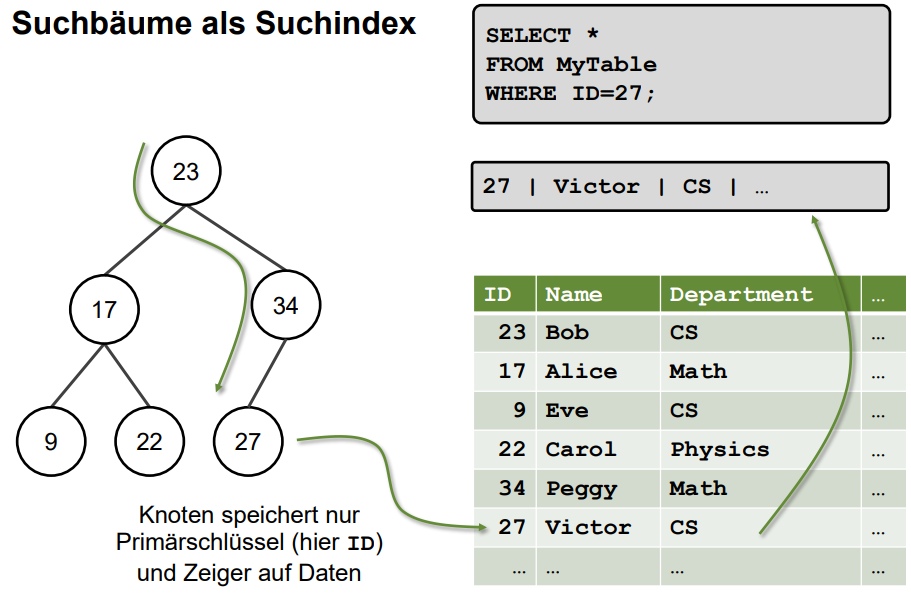
\includegraphics[width=12cm]{suchbaumSuchindex.PNG}
            \end{itemize}
    \end{itemize}

\section{Advanced Data Structures}
\subsection{Rot-Schwarz-Bäume}
    \begin{itemize}
        \item \textbf{Definition}
            \begin{itemize}
                \item Binärer Suchbaum mit Zusatzeigenschaften
                \item Zusatzeigenschaften:
                    \begin{itemize}
                        \item Jeder Knoten hat die Farbe rot oder schwarz
                        \item Die Wurzel ist schwarz
                        \item Wenn ein Knoten rot ist, sind seine Kinder schwarz (\string"Nicht-Rot-Rot-Regel\string")
                        \item Für jeden Knoten hat jeder Pfad zu einem Blatt die selbe Anzahl an gleichen schwarzen Knoten
                    \end{itemize}
                \item Halbblätter im RBT sind schwarz
                \item Schwarzhöhe eines Knoten: \\
                        Eindeutige Anzahl von schwarzen Knoten auf dem Weg zu einem Blatt im Teilbaum des Knoten
                \item Für leeren Baum gibt Schwarzhöhe = 0 ($SH(nil)=0$)
                \item Höhe eines Rot-Schwarz-Baums
                    \begin{itemize}
                        \item $h \leq 2 \cdot log_2(n+1)$  ($n$ Knoten)
                        \item In jedem Unterteilbaum gleiche Anzahl schwarzer Knoten
                        \item Maximal zusätzlich gleiche Anzahl roter Knoten auf diesem Pfad
                        \item Einigermaßen ausbalanciert $\Rightarrow$ Höhe $O(log~n)$
                    \end{itemize}
                \item Alle folgenden Algorithmen arbeiten mithilfe eines Sentinels (zeigt auf sich selbst)
            \end{itemize}
        
        \item \textbf{Einfügen}
            \begin{itemize}
                \item Laufzeit: $\Theta(h)$ ($h$ jedoch $log~n$)
                \item[1.] Finde Elternknoten wie im BST (BST-Einfüge Algorithmus)
                \item[2.] Färbe den neuen Knoten rot
                \item[3.] Wiederherstellen der Rot-Schwarz-Bedingung
                    \begin{itemize}
                        \item[]
                            \begin{minted}[autogobble]{c}
                            fixColorsAfterInsertion(T,z)

                            WHILE z.parent.color == red DO                  // solange der Elternknoten rot ist
                                IF z.parent == z.parent.parent.left THEN    // Linkes Kind (if-Fall)
                                    y = z.parent.parent.right;
                                    IF y != nil AND y.color == red THEN     // Fall 1
                                        z.parent.color = block;
                                        y.color = black;
                                        z.parent.parent.color = red;
                                        z = z.parent.parent;                // rekursiv nach oben weiterführen
                                    ELSE                                    // Fall 2
                                        IF z == z.parent.right THEN         // Zwischenfall (2.1)
                                            z = z.parent;
                                            rotateLeft(T,z);
                                        z.parent.color = black;
                                        z.parent.parent.color = red;
                                        rotateRight(T, z.parent.parent);
                                ELSE                                        // Rechtes Kind (else-Fall)
                                    // Tauschen von rechts und links
                                T.root.color = black;                       // Setzen der Wurzel auf Schwarz
                            \end{minted}
                    \end{itemize}
                \item Hilfsmethode \texttt{rotateLeft}
                    \begin{itemize}
                        \item[] 
                            \begin{minted}[autogobble]{c}
                            rotateLeft(T,x)
                            
                            y = x.right;
                            x.right = y.left;
                            IF y.left != nil THEN
                                y.left.parent = x;
                            y.parent = x.parent;
                            IF x.parent == T.sent THEN
                                T.root = y;
                            ELSE
                                IF x == x.parent.left THEN
                                    x.parent.left = y;
                                ELSE
                                    x.parent.right = y;
                            y.left = x;
                            x.parent = y;
                            \end{minted}
                    \end{itemize}
            \end{itemize}

        \item \textbf{Löschen}
            \begin{itemize}
                \item Laufzeit: $O(h) = O(log~n)$
                \item analog zum binären Suchbaum, aber neue Node erbt Farbe der alten Node
                \item Wenn "neue" Node schwarz war $\Rightarrow$ Fixup
                \item Verschiedene Fälle, die auch gegenseitig Voraussetzungen füreinander sind 
                \item Da das Ganze jedoch etwas umfangreicher ist, findet es sich nicht hier in der Zusammenfassung
            \end{itemize}
        
        \item \textbf{Worst-Case-Laufzeiten}
            \begin{itemize}
                \item {\makebox[2cm][l]{Einfügen: }} $\Theta(log~n)$
                \item {\makebox[2cm][l]{Löschen: }} $\Theta(log~n)$
                \item {\makebox[2cm][l]{Suchen: }} $\Theta(log~n)$
            \end{itemize}
    \end{itemize}

\subsection{AVL-Bäume}
    \begin{itemize}
        \item \textbf{Definition:}
            \begin{itemize}
                \item $h \leq 1.441 \cdot log~n$ (optimierte Konstanten - 1,441 vs 2 (RBT))
                \item Binärer Suchbaum
                \item Allerdings Balance in jedem Knoten nur $-1,0,1$
                \item Balance für $x$: $B(x)$ = Höhe(rechter Teilbaum) - Höhe(linker Teilbaum)
                \item[] 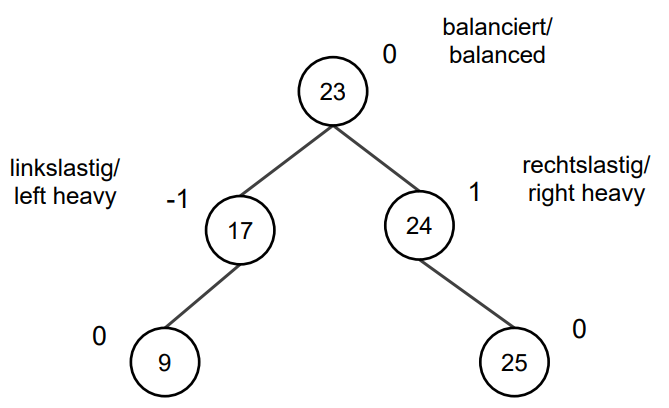
\includegraphics[width=8cm]{avlbaum.PNG}
            \end{itemize}
        
        \item \textbf{AVL vs. Rot-Schwarz}
            \begin{itemize}
                \item AVL:
                    \begin{itemize}
                        \item Einfügen und Löschen verletzen in der Regel öfter die Baum-Bedingung
                        \item Aufwendiger zum Rebalancieren
                    \end{itemize}
                \item Rot-Schwarz:
                    \begin{itemize}
                        \item Suchen dauert evtl. länger
                    \end{itemize}
                \item Konklusion:
                    \begin{itemize}
                        \item AVL geeigneter, wenn mehr Such-Operationen und weniger Einfügen und Löschen
                    \end{itemize}
                \item Gemeinsamkeiten:
                    \item AVL $\subset$ Rot-Schwarz
                    \item AVL Baum $\Rightarrow$ Rot-Schwarz-Baum mit Höhe $\left \lceil \frac{h+1}{2} \right \rceil$
                    \item Für jede Höhe $h \geq 3$ gibt es einen RBT, der kein AVL-Baum ist (AVL $\neq$ RBT)
            \end{itemize}

        \item \textbf{Einfügen}
            \begin{itemize}
                \item Einfügen funktioniert wie beim Binary Search Tree mit Sentinel
                \item Erfordert danach jedoch Rebalancieren weiter oben im Baum
                \item Rebalancieren: (verschiedene Fälle)
                \item[]
                    \begin{minipage}{0.45\textwidth}
                        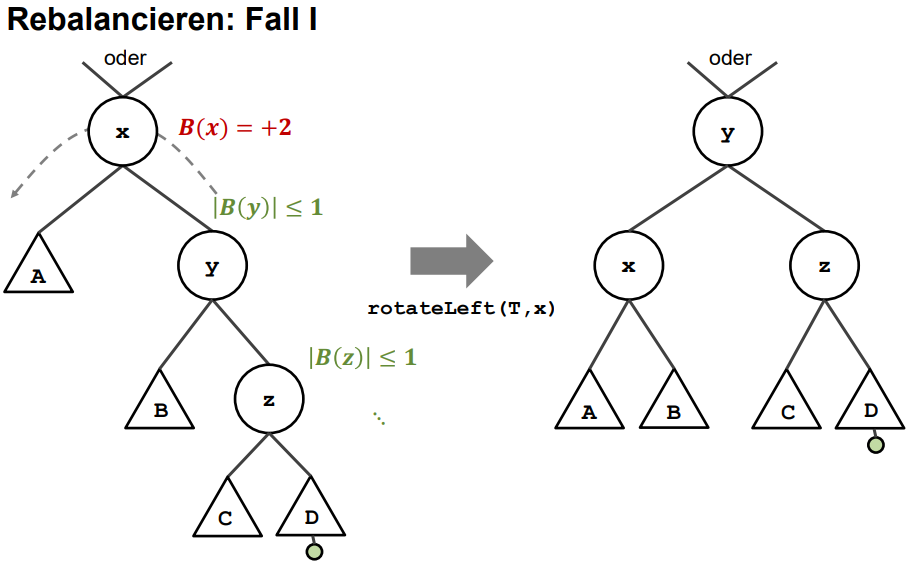
\includegraphics[width=7cm]{avlcase1.PNG}
                    \end{minipage}
                    \begin{minipage}{0.45\textwidth}
                        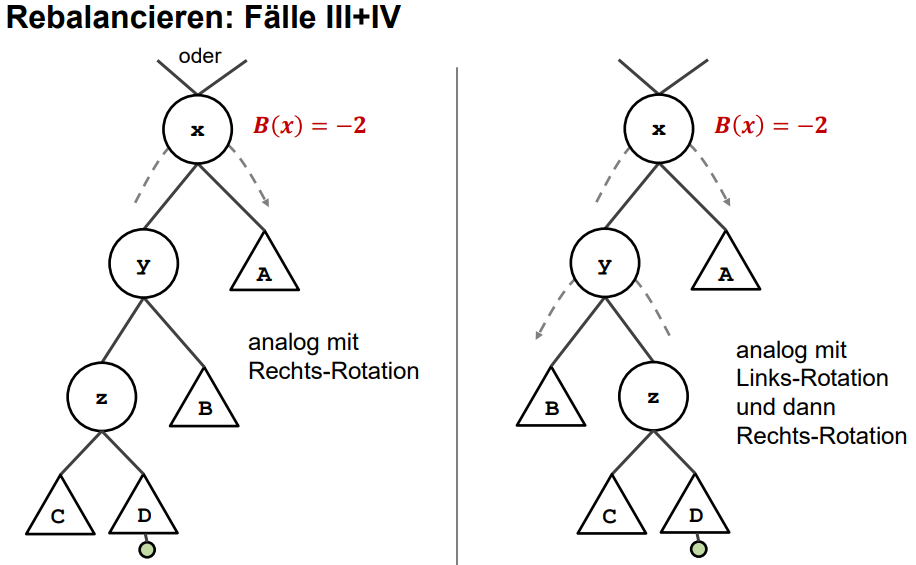
\includegraphics[width=7cm]{avlcase34.PNG} 
                    \end{minipage}
                \item[]
                    \begin{minipage}{0.45\textwidth}
                        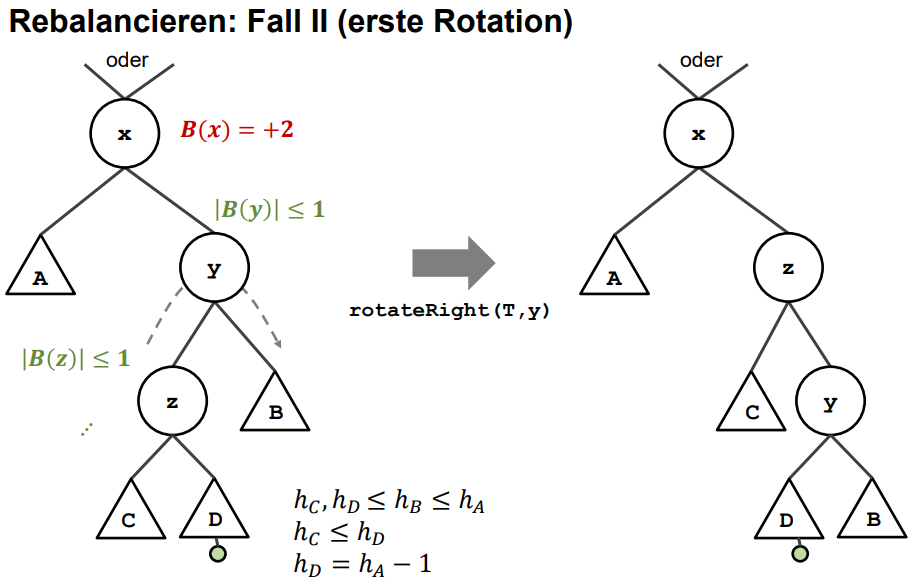
\includegraphics[width=7cm]{avlcase2_1.PNG}
                    \end{minipage}
                    \begin{minipage}{0.45\textwidth}
                        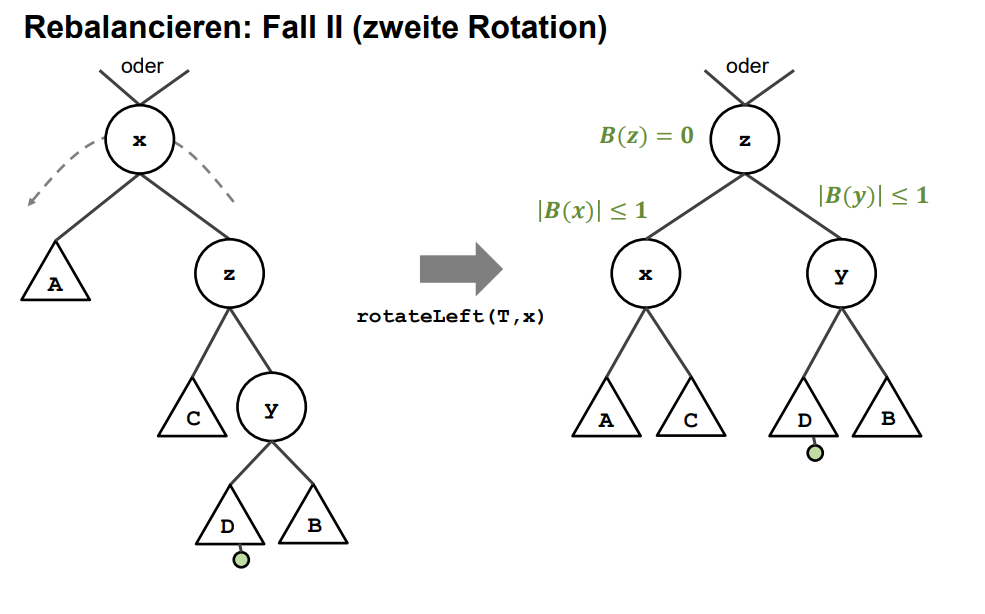
\includegraphics[width=7cm]{avlcase2_2.PNG}
                    \end{minipage}
            \end{itemize}

        \item \textbf{Löschen}
            \begin{itemize}
                \item Analog zum binären Suchbaum
                \item Rebalancieren bis eventuell in die Wurzel notwendig
            \end{itemize}

        \item \textbf{Worst-Case-Laufzeiten}
            \begin{itemize}
                \item {\makebox[2cm][l]{Einfügen: }} $\Theta(log~n)$
                \item {\makebox[2cm][l]{Löschen: }} $\Theta(log~n)$
                \item {\makebox[2cm][l]{Suchen: }} $\Theta(log~n)$
                \item theoretisch bessere Konstanten als RBT
                \item in Praxis aber nur unwesentlich schneller
            \end{itemize}
            
    \end{itemize}

\subsection{Splay-Bäume}
    \begin{itemize}
        \item \textbf{Definition}
            \begin{itemize}
                \item selbst-organisierende Listen
                \item Ansatz: Einmal angefragte Werte werdeb wahrs. noch öfter angefragt
                \item Angefragte Werte nach oben schieben
                \item Splay-Bäume sind Untermenge von BST
            \end{itemize}
        
        \item \textbf{Splay-Operationen}
            \begin{itemize}
                \item Suchen oder Einfügen: Spüle gesuchten oder neu eingefügten Knoten an die Wurzel
                \item Splay: (Folge von Zig-,Zig-Zig-, Zig-Zag-Operationen)
                \item []
                    \begin{minted}[autogobble]{c}
                    splay(T,z)

                    WHILE z != T.root DO
                        IF z.parent.parent == nil THEN
                            zig(T,z);
                        ELSE
                            IF z == z.parent.parent.left.left OR
                               z == z.parent.parent.right.right THEN
                               zigZig(T,z);
                            ELSE
                                zigZag(T,z);
                    \end{minted}
                \item[]
                \item[] \includegraphics[width=9cm]{zigzag.PNG}
                \item[] \includegraphics[width=9cm]{zigzig.PNG}
                \item[] \includegraphics[width=9cm]{zig.PNG}
            \end{itemize}
        
        \item \textbf{Suchen}
            \begin{itemize}
                \item Laufzeit: $O(h)$
                \item Suche des Knotens wie im BST
                \item Hochspülen des gefundenen Knotens (alternativ zuletzt besuchter Knoten, falls nicht gefunden)
            \end{itemize}

        \item \textbf{Einfügen}
            \begin{itemize}
                \item Laufzeit: $O(h)$
                \item Suche der Position wie im BST
                \item Einfügen und danach hochspülen des eingefügten Knotens
            \end{itemize}    

        \item \textbf{Löschen}
            \begin{itemize}
                \item Laufzeit: $O(h)$
                \item[1.] Spüle gesuchten Knoten per Splay-Operation nach oben
                \item[2.] Lösche den gesuchten Knoten (Wenn einer der beiden entstehenden Teilbäume leer, dann fertig)
                \item[3.] Spüle den größten Knoten im linken Teilbaum nach oben (kann kein rechtes Kind haben)
                \item[4.] Hänge rechten Teilbaum an größten Knoten aus 3. an   
            \end{itemize}
        
        \item \textbf{Laufzeit Splay-Bäume}
            \begin{itemize}
                \item Amortisierte Laufzeit: Laufzeit pro Operation über mehrere Operationen hinweg
                \item Worst-Case-Laufzeit pro Operation: $O(log_n~n)$
            \end{itemize}
    \end{itemize}

\subsection{Binäre Max-Heaps}
    \begin{itemize}
        \item \textbf{Definition}
            \begin{itemize}
                \item Heaps sind keine BSTs
                \item Eigenschaften binäre Max-Heaps:
                    \begin{itemize}
                        \item bis auf das unterste Level vollständig und dort von links gefüllt ist
                        \item Für alle Knoten gilt: \texttt{x.parent.key $\geq$ x.key}
                        \item Maximum des Heaps steht damit in der Wurzel
                    \end{itemize}
                \item $h \leq log~n$, da Baum fast vollständig
            \end{itemize}

        \item \textbf{Heaps durch Arrays}
            \begin{itemize}
                \item[] \includegraphics[width=8cm]{heapArr.PNG}
            \end{itemize}

        \item \textbf{Einfügen}
            \begin{itemize}
                \item Idee: Einfügen und danach Vertauschen nach oben, bis Max-Eigenschaft wieder erfüllt ist
                \item Laufzeit: $O(h) = O(log~n)$
                \item[]
                    \begin{minted}[autogobble]{c}
                    insert(H,k) // als unbeschränktes Array

                    H.length = H.length + 1;
                    H.A[H.length-1] = k;

                    i = H.length - 1;
                    WHILE i > 0 AND H.A[i] > H.A[i.parent]
                        SWAP(H.A, i, i.parent);
                        i = i.parent;
                    \end{minted}
            \end{itemize}

        \item \textbf{Lösche Maximum}
            \begin{itemize}
                \item[1.] Ersetze Maximum durch "letztes" Blatt
                \item[2.] Vertausche Knoten durch Maximum der beiden Kinder (\texttt{heapify})
                \item[]
                    \begin{minipage}{0.4\textwidth}
                        \includegraphics[width=6cm]{heapDelete.PNG}
                    \end{minipage} 
                    \begin{minipage}{0.5\textwidth}
                        \begin{minted}[autogobble]{c}
                        extract-max(H)

                        IF isEmpty(H) THEN return error 'underflow';
                        ELSE
                            max = H.A[0];
                            H.A[0] = H.A[H.length - 1];
                            H.length = H.length - 1;
                            heapify(H, 0);
                            return max;
                        \end{minted}
                    \end{minipage}
                \item[]
                    \begin{minted}[autogobble]{c}
                    heapify(H, i)

                    maxind = i;
                    IF i.left < H.length AND H.A[i]<H.A[i.left] THEN
                        maxind = i.left;
                    IF i.right < H.length AND H.A[maxind]<H.A[i.right] THEN
                        maxind = i.right;

                    IF maxind != i THEN
                        SWAP(H.A, i, maxind);
                        heapify(H, maxind);
                    \end{minted}
            \end{itemize}

        \item \textbf{Heap-Konstruktion aus Array}
            \begin{itemize}
                \item Blätter sind für sich triviale Max-Heaps
                \item Bauen von Max-Heaps für Teilbäume mithilfe Rekursion per \texttt{heapify} 
                \item (Array nicht unbedingt in richtiger Reihenfolge)
                \item[]
                    \begin{minted}[autogobble]{c}
                    buildHeap(H.A) // Array in H.A

                    H.length = A.length;
                    FOR i = ceil((H.length-1)/2) - 1 DOWNTO 0 DO
                        heapify(H.A,i);
                    \end{minted}
            \end{itemize}

        \item \textbf{Heap-Sort}
            \begin{itemize}
                \item Idee: Bauen des Heaps aus Array und dann Extraktion des Maximums
                \item[]
                    \begin{minted}[autogobble]{c}
                    heapSort(H.A)

                    buildHeap(H.A)                  // Bauen des Heaps
                    WHILE !isEmpty(H) DO
                        PRINT extract-max(H);       // Ausgabe des Maximums bis Heap leer ist
                    \end{minted}
            \end{itemize}
    \end{itemize}

\subsection{B-Bäume}
    \begin{itemize}
        \item \textbf{Definition}
            \begin{itemize}
                \item Jeder B-Baum hat einen angebenen Grad also z.B. $t=2$
                \item Eigenschaften:
                    \begin{itemize}
                        \item Wurzel zwischen $[1,...,2t-1]$ Werte
                        \item Knoten zwischen $[t-1,...2t-1]$ Werte
                        \item Werte innerhalb eines Knotens aufsteigend geordnet
                        \item Blätter haben alle die gleiche Höhe
                        \item Jeder innere Knoten mit $n$ Werten hat $n+1$ Kinder, sodass gilt:
                        \item[] $k_0 \leq key[0] \leq k_1 \leq key[1] \leq ... \leq k_{n-1} \leq key[n-1] \leq k_n$
                    \end{itemize}
                \item[] \includegraphics[width=9cm]{bbaum.PNG}
                \item Höhe B-Baum: $h \leq log_t \frac{n+1}{2}$ (Grad $t$ und $n$ Werte)
                \item B-Baum wird für größere $t$ flacher
            \end{itemize}
        
        \item \textbf{Suche}
            \begin{itemize}
                \item[] \includegraphics[width=12cm]{bbaumSuche.PNG}
                \item[]
                    \begin{minted}[autogobble]{c}
                    search(x, k)

                    WHILE x != nil DO
                        i = 0;
                        WHILE i < x.n AND x.key[i] < k DO
                            i++;
                        IF i < x.n AND x.key[i] == k THEN
                            return(x, i);
                        ELSE
                            x = x.child[i];
                    return nil;
                    \end{minted}
            \end{itemize}

        \item \textbf{Einfügen}
            \begin{itemize}
                \item Einfügen erfolgt immer in einem Blatt
                \item Falls das Blatt voll ist, muss jedoch gesplittet werden
                \item $\Rightarrow$ Beim Durchlaufen des Baumes an jeder notwendigen (voll) Position splitten
                \item Splitten:
                    \begin{itemize}
                        \item Bricht volle Node auf und fügt mittleren Wert zur Elternnode hinzu
                        \item Aus den anderen Werten entstehen nun jeweils eigene Kinder
                        \item An der Wurzel splitten erzeugt neue Wurzel und erhöht Baumhöhe um eins
                    \end{itemize}
                \item Ablauf zusammengefasst:
                    \begin{enumerate}
                        \item Start bei Wurzel, falls kein Platz mehr splitten
                        \item Durchlaufen des Baumes bis zur richtigen Position und immer, falls voll, splitten
                        \item Einfügen der Node (fertig)
                    \end{enumerate}
                \item[]
                    \begin{minted}[autogobble]{c}
                    insert(T, z)

                    Wenn Wurzel schon 2t-1 Werte, dann splitte Wurzel
                    Suche rekursiv Einfügeposition:
                        Wenn zu besuchendes Kind 2t-1 Werte, splitte es erst
                    Füge z in Blatt ein
                    \end{minted}
            \end{itemize}

        \item \textbf{Löschen}
            \begin{itemize}
                \item Wenn Blatt noch mehr als t-1 Werte, kann der Wert einfach entfernt werden
                \item Allerdings durchlaufen wir hier den Baum auch wieder von oben und stellen gewisse Voraussetzungen her
                \item Durchlaufen des Baumes von oben und Anwendung der folgenden Algorithmen
                \item[]
                    \begin{minipage}{0.25\textwidth}
                        \includegraphics[width=4cm]{bbaumMelt.PNG}
                    \end{minipage}
                    \begin{minipage}{0.65\textwidth}
                        Allgemeines Verschmelzen:
                        \begin{itemize}
                            \item Kind und alle rechten/linken Geschwisterknoten nur $t-1$ Werte
                            \item Wenn Elternknoten vorher min. $t$ Werte
                            \item[] $\Rightarrow$ keine Änderung oberhalb notwendig
                        \end{itemize}
                    \end{minipage}
                \item[]
                    \begin{minipage}{0.25\textwidth}
                        \includegraphics[width=4cm]{bbaumRot.PNG}
                    \end{minipage}
                    \begin{minipage}{0.65\textwidth}
                        Allgemeines Rotieren/Verschieben:
                        \begin{itemize}
                            \item Kind nur $t-1$ Werte
                            \item Geschwister jedoch mehr als $t-1$ Werte
                            \item keine Änderung oberhalb notwendig
                        \end{itemize}
                    \end{minipage}
                \item Code:
                \item[]
                    \begin{minted}[autogobble]{c}
                    delete(T, k)
                    
                    Wenn Wurzel nur 1 Wert und beide Kinder t-1 Werte, 
                    verschmelze Wurzel und Kinder (reduziert Höhe um 1)
                    Suche rekursiv Löschposition:
                        Wenn zu besuchendes Kind nur t-1 Werte, 
                        verschmelze es oder rotiere/verschiebe
                    Entferne Wert k im inneren Knoten/Blatt             
                    // Ohne Probleme, aufgrund vorheriger Anpassung
                    \end{minted}
            \end{itemize}

        \item \textbf{Laufzeiten}
            \begin{itemize}
                \item {\makebox[2cm][l]{Einfügen: }} $\Theta(log_t~n)$
                \item {\makebox[2cm][l]{Löschen: }} $\Theta(log_t~n)$
                \item {\makebox[2cm][l]{Suchen: }} $\Theta(log_t~n)$
                \item Nur vorteilhaft wenn Daten blockweise eingelesen werden
                \item $O$-Notation versteckt hier konstanten Faktor $t$ für Suche innerhalb eines Knotens
            \end{itemize}
    \end{itemize}

\section{Randomized Data Structures}
\subsection{Skip Lists}
    \begin{itemize}
        \item \textbf{Idee}
            \begin{itemize}
                \item Einfügen von \string"Express-Liste\string" mit einigen Elementen
                \item Beginne mit Suche in der Express-Liste mit weniger Elementen
                \item Falls das suchende Element kleiner als nächstes Element in Express-Liste $\Rightarrow$ weiter nach rechts
                \item Falls nicht $\Rightarrow$ Eine Stufe nach unten wandern und dort weiter suchen
                \item[] \includegraphics[width=12cm]{skiplistSuche.PNG}
                \item Verbesserung: Zusätzliche Stufen an Express-Listen 
                \item Anwendung: 
                \begin{itemize}
                    \item Gut für parallele Verarbeitung z.B. Multicore-Systeme (Einfügen und Löschen)
                    \item Dafür logarithmische Laufzeit nur im Durchschnitt
                \end{itemize}
                \item Auswahl von Elementen:
                    \begin{itemize}
                        \item Abhängig von einer gewählten Wahrscheinlichkeit $p$ 
                        \item Element kommt mit Wahrscheinlichkeit $p$ in übergeordnete Liste
                        \item Höhe: $h = O(log_{\frac{1}{p}}n)$
                        \item Anzahl Elemente: $n \Rightarrow pn \Rightarrow p^2n \Rightarrow ...$ (unten nach oben)
                    \end{itemize}
            \end{itemize}

        \item \textbf{Implementierung}
            \begin{itemize}
                \item[]
                    \begin{minipage}{0.5\textwidth}
                        \includegraphics[width=8cm]{skiplistImplement1.PNG}
                    \end{minipage}
                    \begin{minipage}{0.4\textwidth}
                        \includegraphics[width=6cm]{skiplistImplement2.PNG}
                    \end{minipage}
            \end{itemize}

        \item \textbf{Suche}
            \begin{itemize}
                \item Laufzeit ist von Expresslisten abhängig
                \item[]
                    \begin{minted}[autogobble]{c}
                    search(L, k)
                    current = L.head;
                    WHILE current != nil DO
                        IF current.key == k THEN 
                            return current;
                        IF current.next != nil AND current.next.key <= k THEN
                            current = current.next;
                        ELSE
                            current = current.down;
                    return nil;
                    \end{minted}
            \end{itemize}

        \item \textbf{Einfügen}
            \begin{itemize}
                \item Füge auf unterster Ebene ein
                \item Evtl. auf höheren Ebenen mit zufälliger Wahl mithilfe von $p$ auf jeder Ebene
            \end{itemize}

        \item \textbf{Löschen}
            \begin{itemize}
                \item Entferne Vorkommen des Elements aus allen Ebenen
            \end{itemize}
        
        \item \textbf{Laufzeiten}
            \begin{itemize}
                \item {\makebox[2cm][l]{Einfügen: }} $\Theta(log_{\frac{1}{p}}n)$
                \item {\makebox[2cm][l]{Löschen: }} $\Theta(log_{\frac{1}{p}}n)$
                \item {\makebox[2cm][l]{Suchen: }} $\Theta(log_{\frac{1}{p}}n)$
                \item (Im Durchschnitt)
                \item $O$-Notation versteckt konstanten Faktor $\frac{1}{p}$
                \item Speicherbedarf im Durchschnitt: $\frac{n}{1-p}$
            \end{itemize}
    \end{itemize}

\subsection{Hashtables}
    \begin{itemize}
        \item \textbf{Idee}
            \begin{itemize}
                \item[]
                    \begin{minipage}{0.4\textwidth}
                        \includegraphics[width=7cm]{hashtableIdee.PNG}
                    \end{minipage}
                    \begin{minipage}{0.5\textwidth}
                        \begin{itemize}
                            \item Hashfunktion sollte gut verteilen
                            \item $h(x)$ sollte uniform sein
                            \item Unabhängig im Intervall $[0, T.length-1]$ verteilt
                            \item Einfügen mit konstant vielen Array-Operationen
                        \end{itemize}
                    \end{minipage}
                \item[]
                \item[]
                \item[]
                    \begin{minipage}{0.4\textwidth}
                        \includegraphics[width=7cm]{hashtableLinkedList.PNG}
                    \end{minipage}
                    \begin{minipage}{0.5\textwidth}
                        \begin{itemize}
                            \item Kollisionsauflösung z.B. mithilfe von LinkedLists
                            \item Neue Elemente werden vorne angefügt
                            \item Konstante Anzahl an Array-Operationen
                            \item Soviele Schritte wie die Liste lang ist 
                            \item Uniforme Hashfunktion
                            \item[] $\Rightarrow$ $\frac{n}{T.length}$ Einträge pro Liste
                        \end{itemize}
                    \end{minipage}
            \end{itemize}

        \item \textbf{Hash-Funktionen}
            \begin{itemize}
                \item Universelle Hash-Funktion:
                    \begin{itemize}
                        \item Wähle zufällige $a,b \in [0, p - 1]$, $p~prim$, $a \neq 0$
                        \item $h_{a,b}(x)= ((a \cdot x + b)~mod~p)~mod~T.length$
                    \end{itemize}
                \item Krypthographische Hash-Funktionen:
                    \begin{itemize}
                        \item MD5, SHA-1, SHA-2, SHA-3
                        \item $h(x) = MD5(x) mod T.length$
                    \end{itemize}
            \end{itemize}

        \item \textbf{Hashtables vs. Bäume}
            \begin{itemize}
                \item Hashtables:
                    \begin{itemize}
                        \item nur Suche nach bestimmten Wert möglich
                        \item meist größer als zu erwartende Anzahl Einträge
                    \end{itemize}
                \item Bäume:
                    \begin{itemize}
                        \item schnelles Traversieren zu Nachbarn möglich
                        \item Bereichssuche möglich
                    \end{itemize}
            \end{itemize}
        
        \item \textbf{Laufzeiten}
            \begin{itemize}
                \item Wählt mal $T.length = n$ ergibt sich konstante Laufzeit
                \item {\makebox[2cm][l]{Einfügen: }} $\Theta(1)$
                \item {\makebox[2cm][l]{Löschen: }} $\Theta(1)$
                \item {\makebox[2cm][l]{Suchen: }} $\Theta(1)$
                \item (Im Durchschnitt, beim Einfügen sogar im Worst-Case)
                \item Speicherbedarf i.d.R. höher als n, meist ca. $1,33 \cdot n$
            \end{itemize}
    \end{itemize}

\subsection{Bloom-Filter}
    \begin{itemize}
        \item \textbf{Idee}
            \begin{itemize}
                \item Speicherschonende Wörterbucher mit kleinem Fehler
                \item z.B. Vermeidung von schlechten Passwörtern 
                    \begin{enumerate}
                        \item Abspeichern aller schlechten Passwörter in kompakter Form
                        \item Prüfe, ob eingegebenes Passwort im Bloom-Filter
                    \end{enumerate}
                \item z.B. Erkennen von schädlichen Websites (Chrome früher)
            \end{itemize}

        \item \textbf{Erstellen}
            \begin{itemize}
                \item $n$ Elemente $x_0,...,x_{n-1}$
                \item $m$ Bits-Speicher z.B. als Bit-Array
                \item $k$ gute Hash-Funktionen $H_0,...,H_{k-1}$ mit Bildbereich $0,1,...,m-1$
                \item Empfohlene Wahl: $k = \frac{m}{n} \cdot ln2$ (Fehlerrate von ca. $2^{-k}$)
                \item Code:
                \item[]
                    \begin{minted}[autogobble]{c}
                    initBloom(X, BF, H) // H Array of hash functions

                    FOR i = 0 TO BF.length - 1 DO 
                        BF[i] = 0;
                    FOR i = 0 TO X.length - 1 DO
                        FOR j = 0 TO H.length - 1 DO
                            BF[H[j](X[i])] = 1;
                    \end{minted}
                \item[]
                \item[1.] Initialisiere Array mit 0-Einträgen
                \item[2.] Schreibe für jedes Element in jede Bit-Position $H_0(x_i),...,H_{k-1}(x_i)$ eine 1 
                \item[] \includegraphics[width=12cm]{bloomCreate.PNG} 
            \end{itemize}

        \item \textbf{Suche}
            \begin{itemize}
                \item[]
                    \begin{minted}[autogobble]{c}
                    searchBloom(BF, H, y)

                    result = 1;
                    FOR j = 0 TO H.length - 1 DO
                        result = result AND BF[H[j](y)];
                    return result;
                    \end{minted}
                \item[]
                \item Gibt an, dass $y$ im Wörterbuch, falls alle $k$ Einträge für $y$ in $BF=1$ sind
                \item[] \includegraphics[width=12cm]{bloomSearch.PNG}
                \item Eventuell \string"false positives\string" (1, obwohl $y$ nicht im Wörterbuch)
                    \begin{itemize}
                        \item Passiert, falls die Einträge vorher von anderen Werten getroffen wurden
                        \item Daher gute Hashfunktionen und Filtergrö\ss e nicht zu klein
                    \end{itemize}
            \end{itemize}
    \end{itemize}
\end{document}